\documentclass[12pt]{article}

% Geometry
\usepackage[legalpaper, portrait, margin=1in]{geometry}

% Math packages
\usepackage{amsmath}
\usepackage{amssymb}
\usepackage{amsthm}
\usepackage{mathtools}
\usepackage{physics}
% \usepackage{braket}

% Graphics and drawing
\usepackage{graphicx}
\usepackage{tikz}
\usepackage{quantikz} % For quantum circuit drawing
\usepackage{pgfplots}

% Code formatting
\usepackage{minted}

% Layout and formatting
\usepackage{titling}
\usepackage{fancyhdr}
\usepackage{titlesec}
\usepackage{multicol}
\usepackage{xcolor}

% Tables
\usepackage{multirow}
\usepackage{array}
\usepackage{booktabs}
\usepackage{tabularx}


\usemintedstyle{manni}
\graphicspath{ {./figures/} }
\newcommand{\Rlogo}{\protect\includegraphics[height=1.8ex,keepaspectratio]{Rlogo.png}}

% config.tex
\newcommand{\COURSECODE}{QCI402}
\newcommand{\FULLCOURSENAME}{Mathmatical Foundations for Quantum Computing}
\newcommand{\PROFESSORNAME}{Dr. Miao Yu}
\newcommand{\STUDENTNAME}{Mingjia Guan}
\newcommand{\SEMESTER}{Fall}
\newcommand{\YEAR}{2025}
\newcommand{\UNIVERSITY}{Northern University}

%common commands
% math symbols 
\newcommand{\R}{\mathbb{R}}
\newcommand{\C}{\mathbb{C}}
\newcommand{\N}{\mathbb{N}}
\newcommand{\Z}{\mathbb{Z}}
\newcommand{\Q}{\mathbb{Q}}

\newcommand{\Rn}{\mathbb{R}^n}
\newcommand{\Cn}{\mathbb{C}^n}
\newcommand{\Nn}{\mathbb{N}^n}
\newcommand{\Zn}{\mathbb{Z}^n}
\newcommand{\Qn}{\mathbb{Q}^n}

\newcommand{\conj}[1]{{#1}^*}

\newcommand{\od}[2]{\frac{d#1}{d#2}}
\newcommand{\pd}[2]{\frac{\partial#1}{\partial#2}}

\newcommand{\zerovec}{\mathbf{0}}
\newcommand{\vvec}{\mathbf{v}}
\newcommand{\uvec}{\mathbf{u}}
\newcommand{\wvec}{\mathbf{w}}

\newcommand{\ibase}{\mathbf{\hat{i}}}
\newcommand{\jbase}{\mathbf{\hat{j}}}
\newcommand{\kbase}{\mathbf{\hat{k}}}


% Basic quantum states
\newcommand{\ketphi}{\ket{\phi}}
\newcommand{\braphi}{\bra{\phi}}
\newcommand{\ketpsi}{\ket{\psi}}
\newcommand{\brapsi}{\bra{\psi}}

% Common quantum states
\newcommand{\qzero}{\ket{0}}
\newcommand{\qone}{\ket{1}}
\newcommand{\qplus}{\ket{+}}
\newcommand{\qminus}{\ket{-}}
\newcommand{\qpsi}{\ket{\psi}}
\newcommand{\qphi}{\ket{\phi}}
\newcommand{\qchi}{\ket{\chi}}

% Bell states
\newcommand{\bellphi}{\ket{\Phi^+}}
\newcommand{\bellphim}{\ket{\Phi^-}}
\newcommand{\bellpsi}{\ket{\Psi^+}}
\newcommand{\bellpsim}{\ket{\Psi^-}}

% \documentclass[12pt]{article}

\usepackage[legalpaper, portrait, margin=0.75in]{geometry}

\usepackage{amsmath}
\usepackage{amssymb}
\usepackage{amsthm}
\usepackage{physics}
\usepackage{mathtools}
\usepackage{braket}
\usepackage{tikz}
\usepackage{quantikz}
\usepackage{multicol}
\usepackage{xcolor}
\usepackage{fancyhdr}
\usepackage{titlesec}
\usepackage{multirow}
\usepackage{array}
\usepackage{booktabs}
\usepackage{quantikz}
\usepackage{tabularx}


% Page setup
\pagestyle{fancy}
\fancyhf{}
\fancyhead[L]{Quantum Computing LaTeX Quick Reference}
\fancyhead[R]{\thepage}
\setlength{\headheight}{14.5pt}

% Title formatting
\titleformat{\section}{\large\bfseries\color{blue!70!black}}{\thesection}{1em}{}
\titleformat{\subsection}{\normalsize\bfseries\color{blue!50!black}}{\thesubsection}{1em}{}

\title{\textbf{\Large Quantum Computing LaTeX Quick Reference}}
\author{Quick Command Sheet for Quantum Computing Lecture Notes}
\date{}

% =============================================================================
% QUANTUM STATE NOTATION
% =============================================================================

% Basic quantum states
% \newcommand{\ket}{|#1\rangle}
% \newcommand{\bra}{\langle#1|}
% \newcommand{\braket}{\langle#1|#2\rangle}
% \newcommand{\ketbra}{|#1\rangle\langle#2|}
\newcommand{\expectation}[1]{\langle#1\rangle}

\newcommand{\ketphi}{\ket{\phi}}
\newcommand{\braphi}{\bra{\phi}}
\newcommand{\ketpsi}{\ket{\psi}}
\newcommand{\brapsi}{\bra{\psi}}

% Common quantum states
\newcommand{\qzero}{\ket{0}}
\newcommand{\qone}{\ket{1}}
\newcommand{\qplus}{\ket{+}}
\newcommand{\qminus}{\ket{-}}
\newcommand{\qpsi}{\ket{\psi}}
\newcommand{\qphi}{\ket{\phi}}
\newcommand{\qchi}{\ket{\chi}}

% Bell states
\newcommand{\bellphi}{\ket{\Phi^+}}
\newcommand{\bellphim}{\ket{\Phi^-}}
\newcommand{\bellpsi}{\ket{\Psi^+}}
\newcommand{\bellpsim}{\ket{\Psi^-}}

% GHZ and W states
\newcommand{\GHZ}{\ket{\text{GHZ}}}
\newcommand{\Wstate}{\ket{\text{W}}}

% =============================================================================
% QUANTUM OPERATORS AND GATES
% =============================================================================

% Pauli matrices
\newcommand{\sx}{\sigma_x}
\newcommand{\sy}{\sigma_y}
\newcommand{\sz}{\sigma_z}
\newcommand{\si}{\sigma_0}
\newcommand{\pauliX}{\sigma_X}
\newcommand{\pauliY}{\sigma_Y}
\newcommand{\pauliZ}{\sigma_Z}

% Common quantum gates
\newcommand{\hadamard}{H}
\newcommand{\cnot}{\text{CNOT}}
\newcommand{\ccnot}{\text{CCNOT}}
\newcommand{\toffoli}{\text{Toffoli}}
\newcommand{\fredkin}{\text{Fredkin}}
% \newcommand{\swap}{\text{SWAP}}

% Rotation gates
\newcommand{\rx}[1]{R_x(#1)}
\newcommand{\ry}[1]{R_y(#1)}
\newcommand{\rz}[1]{R_z(#1)}
\newcommand{\rn}[2]{R_{\hat{n}}(#1, #2)}

% Phase gates
\newcommand{\phaseS}{S}
\newcommand{\phaseT}{T}
\newcommand{\phaseP}[1]{P(#1)}

% Measurement
% \newcommand{\measure}{\mathcal{M}}
% \newcommand{\proj}[1]{P_{#1}}
\newcommand{\projzero}{\proj{0}}
\newcommand{\projone}{\proj{1}}

% =============================================================================
% QUANTUM OPERATIONS AND PROCESSES
% =============================================================================

% Unitary operations
\newcommand{\unitary}{\mathcal{U}}
\newcommand{\unitarydagger}{\mathcal{U}^\dagger}

% Quantum channels
\newcommand{\channel}{\mathcal{E}}
\newcommand{\noise}{\mathcal{N}}
\newcommand{\depolar}{\mathcal{D}}
\newcommand{\bitflip}{\mathcal{B}}
\newcommand{\phaseflip}{\mathcal{P}}

% Tensor products
\newcommand{\tensor}{\otimes}
% \newcommand{\bigotimes}{\bigotimes}

% Trace operations
% \newcommand{\tr}{\text{Tr}}
\newcommand{\ptr}[1]{\text{Tr}_{#1}}

% =============================================================================
% QUANTUM INFORMATION MEASURES
% =============================================================================

% Entropies
\newcommand{\entropy}[1]{H(#1)}
\newcommand{\condentropy}[2]{H(#1|#2)}
\newcommand{\mutualinfo}[2]{I(#1:#2)}
\newcommand{\vonneumann}[1]{S(#1)}

% Distances and fidelities
\newcommand{\fidelity}[2]{F(#1, #2)}
\newcommand{\tracedist}[2]{D(#1, #2)}

% =============================================================================
% QUANTUM ALGORITHMS
% =============================================================================

% Algorithm names
\newcommand{\QFT}{\text{QFT}}
\newcommand{\iQFT}{\text{QFT}^{-1}}
\newcommand{\grover}{\text{Grover}}
\newcommand{\shor}{\text{Shor}}

% Oracle notation
\newcommand{\oracle}{O}
\newcommand{\oraclef}{O_f}
\newcommand{\oracleg}{O_g}

% Amplitudes
\newcommand{\amp}[1]{\alpha_{#1}}
\newcommand{\betamp}[1]{\beta_{#1}}

% =============================================================================
% QUANTUM ERROR CORRECTION
% =============================================================================

% Stabilizers
\newcommand{\stab}{\mathcal{S}}
\newcommand{\stabgen}{g}
\newcommand{\syndrome}{s}

% Error operators
\newcommand{\error}{E}
\newcommand{\errorX}{X}
\newcommand{\errorY}{Y}
\newcommand{\errorZ}{Z}

% Code spaces
\newcommand{\codespace}{\mathcal{C}}
\newcommand{\codeword}{\ket{\overline{\psi}}}

% =============================================================================
% QUANTUM COMPLEXITY
% =============================================================================

% Complexity classes
\newcommand{\BQP}{\text{BQP}}
\newcommand{\QMA}{\text{QMA}}
\newcommand{\QPSPACE}{\text{QPSPACE}}

% =============================================================================
% QUANTUM CIRCUITS AND DIAGRAMS
% =============================================================================

% Circuit elements (for use with quantikz)
% \newcommand{\qw}{\qw}
% \newcommand{\gate}[1]{\gate{#1}}
% \newcommand{\ctrl}{\ctrl{1}}
% \newcommand{\targ}{\targ{}}
% \newcommand{\meter}{\meter{}}

% =============================================================================
% MATHEMATICAL UTILITIES
% =============================================================================

% Complex numbers
\newcommand{\ii}{\mathrm{i}}
% \newcommand{\real}{\text{Re}}
\newcommand{\imag}{\text{Im}}
\newcommand{\conj}[1]{#1^*}

% Matrix operations
% \newcommand{\rank}{\text{rank}}
\newcommand{\nullspace}{\text{null}}
\newcommand{\colspace}{\text{col}}
\newcommand{\rowspace}{\text{row}}

% Probability
\newcommand{\prob}[1]{\text{Pr}[#1]}
\newcommand{\expect}[1]{\mathbb{E}[#1]}
% \newcommand{\var}[1]{\text{Var}[#1]}

% Sets
\newcommand{\hilbert}{\mathcal{H}}
\newcommand{\density}{\mathcal{D}}
\newcommand{\positive}{\mathcal{P}}

% =============================================================================
% QUANTUM PHYSICS NOTATION
% =============================================================================

% Time evolution
\newcommand{\hamiltonian}{\mathcal{H}}
\newcommand{\timeevol}[1]{e^{-\ii #1 t/\hbar}}
% \newcommand{\hbar}{\hbar}

% Angular momentum
\newcommand{\angmom}{\mathbf{J}}
\newcommand{\spin}{\mathbf{S}}
\newcommand{\orbital}{\mathbf{L}}

% Commutators and anticommutators
% \newcommand{\comm}[2]{[#1, #2]}
\newcommand{\anticomm}[2]{\{#1, #2\}}

% =============================================================================
% ENVIRONMENTS FOR QUANTUM COMPUTING
% =============================================================================

% Theorem-like environments (already defined in main template)
% Additional quantum-specific environments
\theoremstyle{definition}
\newtheorem{algorithm}{Algorithm}[section]
\newtheorem{protocol}{Protocol}[section]
\newtheorem{circuit}{Circuit}[section]

\theoremstyle{remark}
\newtheorem{quantum-note}{Quantum Note}[section]
\newtheorem{classical-note}{Classical Note}[section]

\begin{document}
\maketitle
\thispagestyle{fancy}

\begin{multicols}{2}

\section{Basic Quantum State Notation}

\subsection{State Vectors}
\begin{alignat}{2}
\text{Ket:}          &\quad && \ket{\psi} \text{ or } \qpsi \\
\text{Bra:}          &\quad && \bra{\psi} \\
\text{Braket:}       &\quad && \braket{\psi | \phi} \\
\text{Outer product:}&\quad && \ketbra{\psi}{\phi} \\
\text{Expectation:}  &\quad && \expectation{A} = \braket{\psi}{A|\psi}
\end{alignat}

\subsection{Common States}
\begin{alignat}{2}
\text{Computational basis:} &\quad && \qzero, \qone \\
\text{Superposition:}       &\quad && \qplus = \frac{1}{\sqrt{2}}(\qzero + \qone) \\
                             &\quad && \qminus = \frac{1}{\sqrt{2}}(\qzero - \qone) \\
\text{Bell states:}         &\quad && \bellphi, \bellphim, \bellpsi, \bellpsim \\
\text{Multi-qubit:}         &\quad && \GHZ, \Wstate
\end{alignat}


\section{Quantum Gates and Operations}

\subsection{Single-Qubit Gates}
\begin{alignat}{2}
\text{Pauli matrices:} &\quad && \pauliX, \pauliY, \pauliZ \\
\text{Hadamard:}       &\quad && \hadamard \\
\text{Phase gates:}    &\quad && \phaseS, \phaseT, \phaseP{\theta} \\
\text{Rotations:}      &\quad && \rx{\theta}, \ry{\theta}, \rz{\theta}
\end{alignat}

\subsection{Multi-Qubit Gates}
\begin{alignat}{2}
\text{CNOT:}     &\quad && \cnot \\
\text{Toffoli:}  &\quad && \toffoli \text{ or } \ccnot \\
\text{Fredkin:}  &\quad && \fredkin \\
\text{SWAP:}     &\quad && \text{SAWP}
\end{alignat}

\section{Quantum Measurements}

\begin{alignat}{2}
\text{Measurement operator:} &\quad && \mathcal{M} \\
\text{Projectors:}           &\quad && \projzero, \projone, \P_{i} \\
\text{Probability:}          &\quad && \prob{i} = \braket{\psi}{\proj{i}|\psi}
\end{alignat}

% \newcommand{\measure}{\mathcal{M}}
% \newcommand{\proj}[1]{P_{#1}}


\section{Quantum Channels and Noise}

\begin{alignat}{2}
\text{General channel:} &\quad && \channel(\rho) \\
\text{Depolarizing:}    &\quad && \depolar_p(\rho) \\
\text{Bit flip:}        &\quad && \bitflip_p(\rho) \\
\text{Phase flip:}      &\quad && \phaseflip_p(\rho)
\end{alignat}


\section{Quantum Information Measures}

\begin{alignat}{2}
\text{Von Neumann entropy:} &\quad && \vonneumann{\rho} \\
\text{Conditional entropy:} &\quad && \condentropy{A}{B} \\
\text{Mutual information:}  &\quad && \mutualinfo{A}{B} \\
\text{Fidelity:}             &\quad && \fidelity{\rho}{\sigma} \\
\text{Trace distance:}       &\quad && \tracedist{\rho}{\sigma}
\end{alignat}


\section{Quantum Algorithms}

\subsection{Fourier Transform}
\begin{alignat}{2}
\text{QFT:}         &\quad && \QFT\ket{x} = \frac{1}{\sqrt{N}} \sum_{k=0}^{N-1} e^{2\pi i xk/N}\ket{k} \\
\text{Inverse QFT:} &\quad && \iQFT
\end{alignat}

\subsection{Oracles}
\begin{alignat}{2}
\text{Boolean oracle:} &\quad && \oraclef\ket{x}\ket{y} = \ket{x}\ket{y \oplus f(x)} \\
\text{Phase oracle:}   &\quad && \oraclef\ket{x} = (-1)^{f(x)}\ket{x}
\end{alignat}

\section{Error Correction}

\begin{alignat}{2}
\text{Stabilizer group:}  &\quad && \stab = \langle g_1, g_2, \ldots, g_k \rangle \\
\text{Syndrome:}          &\quad && \syndrome = (s_1, s_2, \ldots, s_k) \\
\text{Code space:}        &\quad && \codespace \\
\text{Logical codeword:}  &\quad && \codeword
\end{alignat}


\section{Mathematical Utilities}

\subsection{Complex Numbers}
\begin{alignat}{2}
\text{Imaginary unit:}     &\quad && \ii \\
\text{Real part:}          &\quad && \real(z) \\
\text{Imaginary part:}     &\quad && \imag(z) \\
\text{Complex conjugate:}  &\quad && \conj{z}
\end{alignat}

\subsection{Linear Algebra}
\begin{alignat}{2}
\text{Tensor product:}  &\quad && A \tensor B \\
\text{Trace:}           &\quad && \tr(A) \\
\text{Partial trace:}   &\quad && \ptr{B}(\rho_{AB}) \\
\text{Rank:}            &\quad && \rank(A)
\end{alignat}

\subsection{Probability}
\begin{alignat}{2}
\text{Probability:}  &\quad && \prob{\text{event}} \\
\text{Expectation:}  &\quad && \expect{X} \\
\text{Variance:}     &\quad && \var{X}
\end{alignat}

\end{multicols}


\section{Circuit Notation (with quantikz)}

Basic circuit elements:
\begin{verbatim}
\begin{quantikz}
\lstick{$\ket{0}$} & \gate{H} & \ctrl{1} & \meter{} \\
\lstick{$\ket{0}$} & \qw & \targ{} & \qw
\end{quantikz}
\end{verbatim}

\section{Complexity Classes}

\begin{alignat}{2}
\text{Bounded-error quantum polynomial:} &\quad && \BQP \\
\text{Quantum Merlin-Arthur:}           &\quad && \QMA \\
\text{Quantum polynomial space:}        &\quad && \QPSPACE
\end{alignat}


\section{Usage Examples}

\subsection{Quantum Teleportation Protocol}
The quantum teleportation protocol transfers the state $\qpsi = \alpha\qzero + \beta\qone$ using the following steps:

\begin{protocol}
\begin{enumerate}
\item Alice and Bob share the Bell state $\bellphi = \frac{1}{\sqrt{2}}(\ket{00} + \ket{11})$
\item Alice performs a Bell measurement on her qubit and the qubit to be teleported
\item Alice sends the classical result to Bob
\item Bob applies the appropriate correction based on Alice's measurement
\end{enumerate}
\end{protocol}

\subsection{Grover's Algorithm}
Grover's algorithm amplifies the amplitude of marked states:

\begin{algorithm}
\begin{enumerate}
\item Initialize: $\ket{\psi_0} = \frac{1}{\sqrt{N}}\sum_{x=0}^{N-1}\ket{x}$
\item Apply $G = -\hadamard^{\tensor n}\proj{0}^{\tensor n}\hadamard^{\tensor n}\oraclef$ for $O(\sqrt{N})$ iterations
\item Measure to obtain the marked state with high probability
\end{enumerate}
\end{algorithm}

\subsection{Quantum Error Correction Example}
The 3-qubit bit flip code protects against single bit flip errors:

\begin{circuit}
Encoding: $\ket{0} \rightarrow \ket{000}$, $\ket{1} \rightarrow \ket{111}$

Syndrome measurement: $s_1 = Z_1Z_2$, $s_2 = Z_2Z_3$
\end{circuit}

\section{Common Quantum Gates}

\begin{table}[h!]
\centering
\renewcommand{\arraystretch}{1.6}
\begin{tabularx}{\textwidth}{X X}
% --- Left column: Single-Qubit ---
\begin{tabular}{cl}
\toprule
\textbf{Gate} & \textbf{Matrix} \\
\midrule
Hadamard ($H$) &
$\dfrac{1}{\sqrt{2}} \begin{bmatrix}
1 & 1 \\
1 & -1
\end{bmatrix}$ \\
Identity ($I$) &
$\begin{bmatrix}
1 & 0 \\
0 & 1
\end{bmatrix}$ \\
Phase ($S$) &
$\begin{bmatrix}
1 & 0 \\
0 & i
\end{bmatrix}$ \\
T-gate ($T$) &
$\begin{bmatrix}
1 & 0 \\
0 & e^{i\pi/4}
\end{bmatrix}$ \\
NOT ($X$) &
$\begin{bmatrix}
0 & 1 \\
1 & 0
\end{bmatrix}$ \\
Y-gate ($Y$) &
$\begin{bmatrix}
0 & -i \\
i & 0
\end{bmatrix}$ \\
Z-gate ($Z$) &
$\begin{bmatrix}
1 & 0 \\
0 & -1
\end{bmatrix}$ \\
Rotation $R(\theta)$ / Phase $P(\theta)$ &
$\begin{bmatrix}
1 & 0 \\
0 & e^{i\theta}
\end{bmatrix}$ \\
\bottomrule
\end{tabular}
&
% --- Right column: Multi-Qubit ---
\begin{tabular}{cl}
\toprule
\textbf{Gate} & \textbf{Matrix} \\
\midrule
CNOT ($CX$) &
$\begin{bmatrix}
1 & 0 & 0 & 0 \\
0 & 1 & 0 & 0 \\
0 & 0 & 0 & 1 \\
0 & 0 & 1 & 0
\end{bmatrix}$ \\
Controlled-Z ($CZ$) &
$\begin{bmatrix}
1 & 0 & 0 & 0 \\
0 & 1 & 0 & 0 \\
0 & 0 & 1 & 0 \\
0 & 0 & 0 & -1
\end{bmatrix}$ \\
Controlled-$U$ ($CU$) &
$\begin{bmatrix}
1 & 0 & 0 & 0 \\
0 & 1 & 0 & 0 \\
0 & 0 & U_{00} & U_{01} \\
0 & 0 & U_{10} & U_{11}
\end{bmatrix}$ \\
SWAP &
$\begin{bmatrix}
1 & 0 & 0 & 0 \\
0 & 0 & 1 & 0 \\
0 & 1 & 0 & 0 \\
0 & 0 & 0 & 1
\end{bmatrix}$ \\
Toffoli (CCNOT) &
\scriptsize
$\begin{bmatrix}
1 & 0 & 0 & 0 & 0 & 0 & 0 & 0 \\
0 & 1 & 0 & 0 & 0 & 0 & 0 & 0 \\
0 & 0 & 1 & 0 & 0 & 0 & 0 & 0 \\
0 & 0 & 0 & 1 & 0 & 0 & 0 & 0 \\
0 & 0 & 0 & 0 & 1 & 0 & 0 & 0 \\
0 & 0 & 0 & 0 & 0 & 1 & 0 & 0 \\
0 & 0 & 0 & 0 & 0 & 0 & 0 & 1 \\
0 & 0 & 0 & 0 & 0 & 0 & 1 & 0
\end{bmatrix}$
\normalsize \\
\bottomrule
\end{tabular}
\end{tabularx}
\end{table}




\begin{figure}[h]
\centering
\begin{quantikz}
\lstick{$\ket{0}$} & \gate{H} & \ctrl{1} & \meter{} \\
\lstick{$\ket{0}$} & \qw    & \targ{}  & \meter{}
\end{quantikz}
\caption{Quantum circuit for preparing and measuring a Bell state}
\end{figure}



\end{document}

\theoremstyle{definition}
\newtheorem{theorem}{Theorem}[section]
\newtheorem{definition}[theorem]{Definition}
\newtheorem{postulate}[theorem]{Postulate}
\newtheorem{corollary}[theorem]{Corollary}
\newtheorem{lemma}[theorem]{Lemma}

% % alt styling: theorem is separate from rest
% % Theorem: its own counter, resets each section
% \newtheorem{theorem}{Theorem}[section]

% % Create an independent base counter for the "definition group"
% \newtheorem{fact}{\!\!}[section] % invisible title; serves only as a counter

% % Make these share the "fact" counter (not the theorem counter)
% \newtheorem{definition}[fact]{Definition}
% \newtheorem{postulate}[fact]{Postulate}
% \newtheorem{corollary}[fact]{Corollary}
% \newtheorem{lemma}[fact]{Lemma}

\newtheorem*{example}{Example}

\newtheorem*{solution}{Solution}

\title{\COURSECODE\ - \FULLCOURSENAME\ - \UNIVERSITY}
\author{\PROFESSORNAME\ - \STUDENTNAME}
\date{\SEMESTER\ Semester \YEAR}

\begin{document}

\maketitle

\hfill

The underpinnings of all scientific advancements is the ability to express natural phenomena with the art of Mathmatics; this is no different for the subject of Quantum Computing. While the boundaries of quantum computing have been pushed beyond limits in theoretical terms on university blackboards, it has become of great interest to realize the theoretical computational power with the advances of hardware and technology. 

However, these notes mainly concerns itself with the mathmatical underpinnings of quantum computing that the course surrounds itself with. \FULLCOURSENAME takes a scaffolding approach designed to efficiently convey the required theoretical understanding of mathmatics in order to able to learn quantum computing. As of writing, we are basing the notes on verison one of the textbook published in March 2025. In this text, we will primarily be using dirac notation for the expression of vectors, operators, and their interactions. 

\tableofcontents

\break


\section{Summation and Product Notations}

This section primarily focuses on the common notations applied across mathmatics to denote and shorten addition and product notation. 

\subsection{Summation over a single Variable}

The sigma notation is defined as follows

$$\sum_{i=1}^{n}f(i)$$

where we use sigma $\sum$ to represent the sum of a series. For example, the sum of all numbers in a series beginning with $m$ and ending at index $n$ is written as:

$$\sum_{i=m}^{n} a_i = a_m + a_{m+1} + a_{m+2} + \cdots + a_{n-1} + a_n$$

Sums can also be infinite, commonly seen when Sigma looks as follows: $\sum^{\infty}_{i=m}$. Infinite sums are either convergent or divergent. A few of the most common converging infinite sums are as follows:

$$\sum_{i=0}^{\infty} \frac{1}{2^i} = 1 + \frac{1}{2} + \frac{1}{4} + \cdots = 2$$
$$\sum_{i=0}^{\infty}  \frac{1}{i^2} = \frac{1}{1^2} + \frac{1}{2^2} + \frac{1}{3^2} + \cdots = \frac{\pi^2}{6}$$

The first example is an infinite geometric series, and the sum of the first $n$ terms is given by:

$$S_n = \sum_{i=0}^{n} \frac{1}{2^i} = \frac{1 - \frac{1}{2^n}}{1 - \frac{1}{2}}$$

As $n \rightarrow \infty, \frac{1}{2^n} \rightarrow 0$. Consequently, $S_n \rightarrow \frac{1}{1 - \frac{1}{2}} = 2$. A rigorous proof of the second example requires extensive calculus and is not immediately obvious. While any mathmatical symbol can be used for the index of a summation, it is more practical to use something other than $i$ as in the context of complex numbers, $i$ commonly denotes the complex number$\sqrt{-1}$. moreover, sume can also be specified using descriptions. For example, 

$$\sum_{p \in P} f(p) \qquad P \in \mathbb{N^\prime}$$

where $\mathbb{N^\prime}$ is the set of all prime numbers. Summations can also contain parameters other than the index, which results in functions of those parameters. For example the discrete Fourier transform (DFT) is given by

$$\tilde{x}_k = \frac{1}{\sqrt{N}} \sum_{n=0}^{N - 1} x_n e^{- \frac{2 \pi i}{N} kn}, \quad k = 0, 1, \cdots N-1$$

where $x_n$ represents the $N$ values index by $n$ and $\tilde{x}_k$ are the Fourier coefficients. Here, $i$ is the imaginary numebr and $N$ is a positive integer representing the dimension fo the DFT, of which we will cover in greater depth in Chapter 3. The following are some useful summation forumae commonly encountered in quantum computing:

\[
\sum_{i=1}^{n} i = \frac{n(n+1)}{2}
\]

\[
\sum_{i=1}^{n} i^2 = \frac{n(n+1)(2n+1)}{6}
\]

\[
\sum_{i=1}^{n} i^3 = \left(\frac{n(n+1)}{2}\right)^2
\]

\[
\sum_{i=0}^{n} \left(a_0 + id\right) = (n+1)\left(a_0 + \frac{nd}{2}\right) \quad \text{(arithmetic series)}
\]

\[
\sum_{i=0}^{n} a^i = \frac{1 - a^{n+1}}{1 - a} \quad \text{(geometric series)}
\]

\[
(a + b)^n = \sum_{i=0}^{n} \binom{n}{i} a^{n-i} b^i \quad \text{(binomial theorem)}
\]

\[
\frac{1}{1 - x} = \sum_{n=0}^{\infty} x^n = 1 + x + x^2 + x^3 + \cdots \quad (\lvert x \rvert < 1)
\]

\[
\frac{1}{(1-x)^2} = \sum_{n=1}^{\infty} n x^{n-1} = 1 + 2x + 3x^2 + 4x^3 + \cdots \quad (\lvert x \rvert < 1)
\]

\[
\ln(1 + x) = \sum_{n=1}^{\infty} \frac{(-1)^{n+1}}{n} x^n = x - \frac{x^2}{2} + \frac{x^3}{3} - \cdots \quad (\lvert x \rvert < 1)
\]

\[
e^x = \sum_{n=0}^{\infty} \frac{x^n}{n!} = 1 + x + \frac{x^2}{2!} + \frac{x^3}{3!} + \cdots
\]

\[
\sin x = \sum_{n=0}^{\infty} \frac{(-1)^n}{(2n+1)!} x^{2n+1} = x - \frac{x^3}{3!} + \frac{x^5}{5!} - \cdots
\]

\[
\cos x = \sum_{n=0}^{\infty} \frac{(-1)^n}{(2n)!} x^{2n} = 1 - \frac{x^2}{2!} + \frac{x^4}{4!} - \cdots
\]

Below are also a list of the common summations rules and manupulations:

\[
\sum_{i=m}^{n} a_i = \sum_{j=m}^{n} a_j \quad \text{(change of index variable)}
\]

\[
\sum_{i=s}^{t} f(i) = \sum_{n=s}^{t} f(n) \quad \text{(change of index variable)}
\]

\[
\sum_{n=s}^{t} f(n) = \sum_{n=s}^{j} f(n) + \sum_{n=j+1}^{t} f(n) \quad \text{(splitting a sum)}
\]

\[
\sum_{n=s}^{t} f(n) = \sum_{n=0}^{t-s} f(t-n) \quad \text{(reverse order)}
\]

\[
\sum_{n=s}^{t} f(n) = \sum_{n=s+p}^{t+p} f(n-p) \quad \text{(index shift)}
\]

\[
\sum_{n=s}^{t} a \cdot f(n) = a \cdot \sum_{n=s}^{t} f(n) \quad \text{(distributivity)}
\]

\[
\sum_{n=s}^{t} f(n) \pm \sum_{n=s}^{t} g(n) = \sum_{n=s}^{t} \left(f(n) \pm g(n)\right) \quad \text{(commutativity)}
\]


\subsection{Products and other Notations}

Similar to the $\sum$ notation for addition, the $\prod$ (Pi) symbol is also more commonly used to dentoe the product of a series of terms. In this 

$$\prod_{i=m}^{n} a_i = a_m \cdot a_{m+1} \cdot a_{m+2} \cdot \cdots \cdot a_{n-1} \cdot a_n$$ 

for example, the factorial of $n$ is expressed as 

$$\prod_{i=0}^{n} i = n!$$

and the relationship between $\sum$ and $\prod$, which are 

$$b^{\sum_{n=s}^{t} f(n)} = \prod_{n=s}^{t} b^{f(n)}$$

$$\sum_{n=s}^{t} \log_b f(n) = log_b \prod_{n=s}^{t} f(n)$$

It is worth noting that in quantum computing and linear algebra, there are a few special notations such as the modulo-2 sum (bitwise XOR), or in other contexts the direct sum of linear spaces, represented by $\oplus$, and the tensor product represented by $\otimes$.

\subsection{Summation over Multiple Variables}

The double summation over a rectangular array is given by 

\begin{align*}
    \sum_{i=1,j=1}^{n_1, n_2} a_{i,j} &= \sum_{i=1}^{n_1} \sum_{j=1}^{n_2} a_{i, j} = \sum_{j=1}^{n_2} \sum_{i=1}^{n_1} a_{i, j} \\
    &= a_{1, 1} + a_{1, 2} + a_{1, 3} + a_{1, 4} + \cdots + a_{1, n_2} \\
    &+ a_{2, 1} + a_{2, 2} + a_{2, 3} + a_{2, 4} + \cdots + a_{2, n_2} \\
    & + a_{3, 1} + a_{3, 2} + a_{3, 3} + a_{3, 4} + \cdots + a_{3, n_2} \\
    & + a_{4, 1} + a_{4, 2} + a_{4, 3} + a_{4, 4} + \cdots + a_{4, n_2} \\
    & + \cdots \\
    & + a_{n_1, 1} + a_{n_1, 2} + a_{n_1, 3} + a_{n_1, 4} + \cdots + a_{n_1, n_2}
\end{align*}

Here, $\sum_{i=1}^{n_1} \sum_{j=1}^{n_2}$ represents summing over each row first and then summing the results, while $\sum_{j=1}^{n_2} \sum_{i=1}^{n_1}$ will represent summing over the columns and then summing those results. The term $\sum_{i=1,j=1}^{n_1, n_2} a_{i,j}$ represents the summation over the rectangular array, irrespecive of the order. The product of two sums can be expanded into a double sum as follows:

\begin{align*}
\left( \sum_{i=1}^{m} a_i \right) \left( \sum_{j=1}^{n} b_j \right)
    &= (a_1 + a_2 + \cdots + a_m)(b_1 + b_2 + \cdots + b_n) \\
    &=\; a_1b_1 + a_1b_2 + a_1b_3 + a_1b_4 + \cdots + a_1b_n \\
    &+ a_2b_1 + a_2b_2 + a_2b_3 + a_2b_4 + \cdots + a_2b_n \\
    &+ a_3b_1 + a_3b_2 + a_3b_3 + a_3b_4 + \cdots + a_3b_n \\
    &+ \cdots \\
    &+ a_mb_1 + a_mb_2 + a_mb_3 + a_mb_4 + \cdots + a_mb_n \\
    &= \sum_{i=1}^{m} \sum_{j=1}^{n} a_i b_j = \sum_{i=1}^{m} a_i \sum_{j=1}^{n} b_j
\end{align*}

which is actually rather intuitive given how the expansion of the standard expansion of the term $(a+b)^2$ plays out, a more elementary application of the distributive property which the above equation generalizes over. For a triangular matrix, in this case the lower triangular matrix, the sum is given by

\begin{align*}
    \sum_{1 \leq j \leq n}^{} a_{i,j} &= \sum_{i=1}^{n} \sum_{j=1}^{i} a_{i, j} = 
    \sum_{j=1}^{n} \sum_{i=j}^{n} a_{i, j} = 
    \sum_{j=0}^{n-1} \sum_{j=1}^{n-j} a_{i+j, i} \\
    &= a_{1, 1} \\
    & + a_{2, 1} + a_{2, 2}  \\
    & + a_{3, 1} + a_{3, 2} + a_{3, 3} \\
    & + a_{4, 1} + a_{4, 2} + a_{4, 3} + a_{4, 4} \\
    & + \cdots \\
    & + a_{n, 1} + a_{n, 2} + a_{n, 3} + a_{n, 4} + \cdots + a_{n, n}
\end{align*}

where the term $\sum_{1 \leq j \leq n}^{} a_{i,j}$ denotes the summation over all elements in a lower triangular array including the diagonal. The first notation variation will sum up each row to the $i$th element then aggregate while the second notation sums each column starting from the $j$th element downwards then aggregate the sums. The final expression will sum along the diagonal where $j=0$ represents the main diagonal and $j=n-1$ is the first off-diagonal, which is a single term. 

\begin{example}
    Say we would like to expand the product of $\left(1 + x_i\right)$ from $1$ to $n$. We have 

    $$\prod_{i=1}^{n} \left(1 + x_i\right) = 1 + \sum_{k=1}^{n} \left(\sum_{1 \leq i_1 < \cdots < i_k \leq n} \prod_{j=1}^{k} x_{i_j}\right)$$
\end{example}

This formula represents the \textit{multinomial expansion} of a product. When you expand the equation by hand, you get the product

$$\prod_{i=1}^{n} \left(1 + x_i\right) = (1 + x_1)(1 + x_2)\cdots(1 + x_n)$$

If we break this down, we see that the outer summation $\sum_{k=1}^{n}$ will go through each possible summation size in terms of the variables in question, and that the inner summation $\sum_{1 \leq i_1 < \cdots < i_k \leq n}$ will iterate through each possible unique product of the variables. while ensuring that they are unique. Not sure how this works, but if all $x_i$ are the same, then wesee that the equation actually simplifies to a subset of the binomial theorem 

$$(1 + x)^n = \sum_{k=0}^{n} \binom{n}{k} x^k$$

where $\binom{n}{k}$ is the binomial coefficient representing the numebr of ways to choose $k$ elements from a set of $n$ distinct elements.

\break

\section{Trigonometry}

You can't escape this.

\subsection{Definitions}

I mean, where do I start? The basic trigonometric functions are defined as the ratios between the angles of a right triangle. I will not show how these ratios remain the same given the same angle, nor will I go into great mathmatical detail of how to prove these items. However, we still have to go over this. Don't ask me why. 

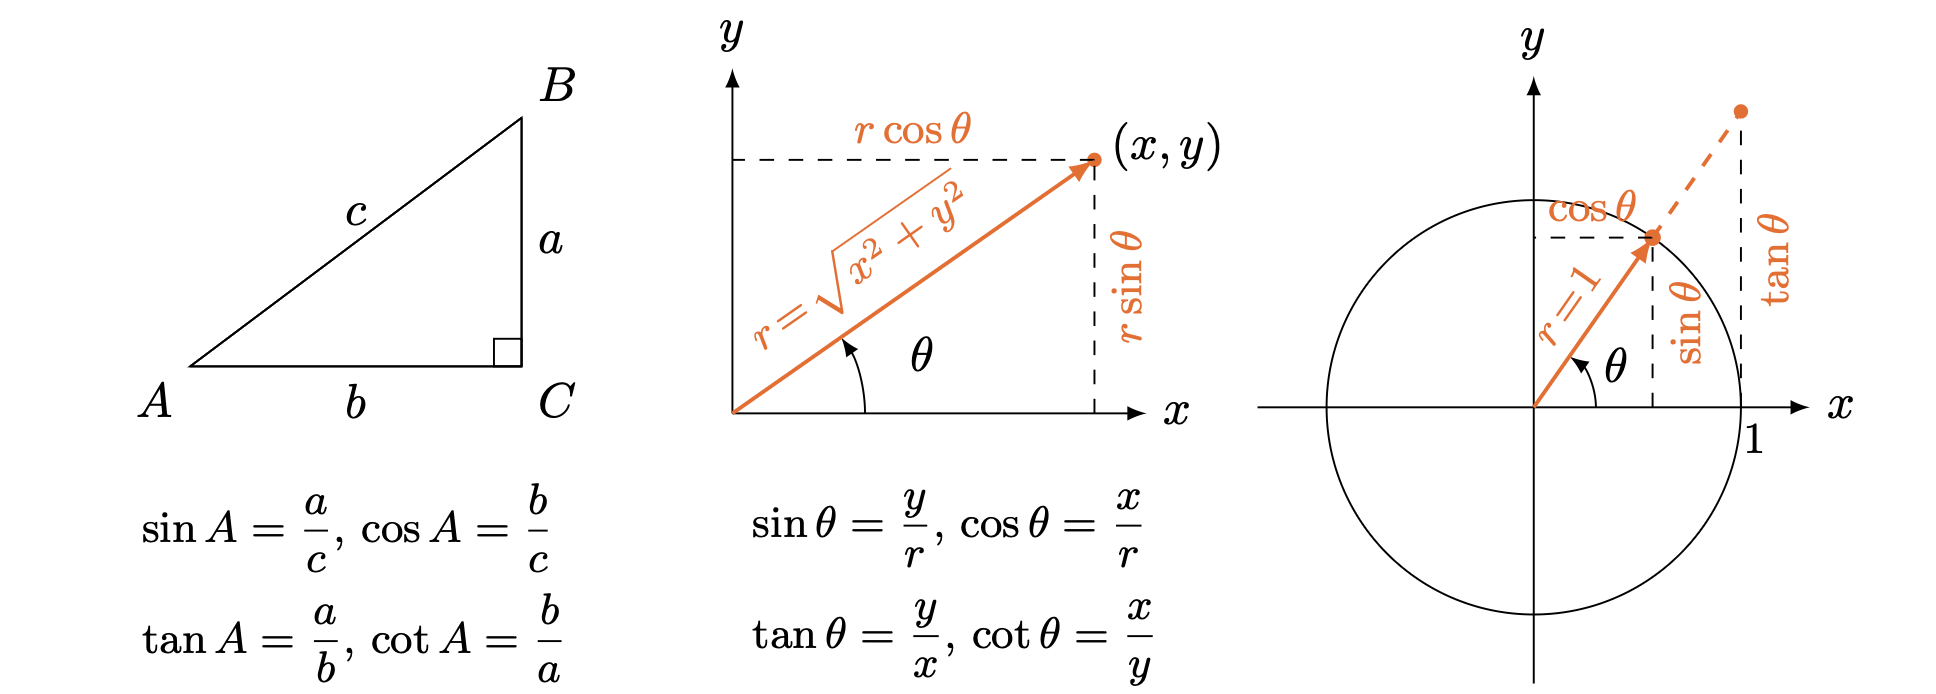
\includegraphics[width=\textwidth]{2_trig0}

The functions of trigonometric functions can also be plotted out as follows:

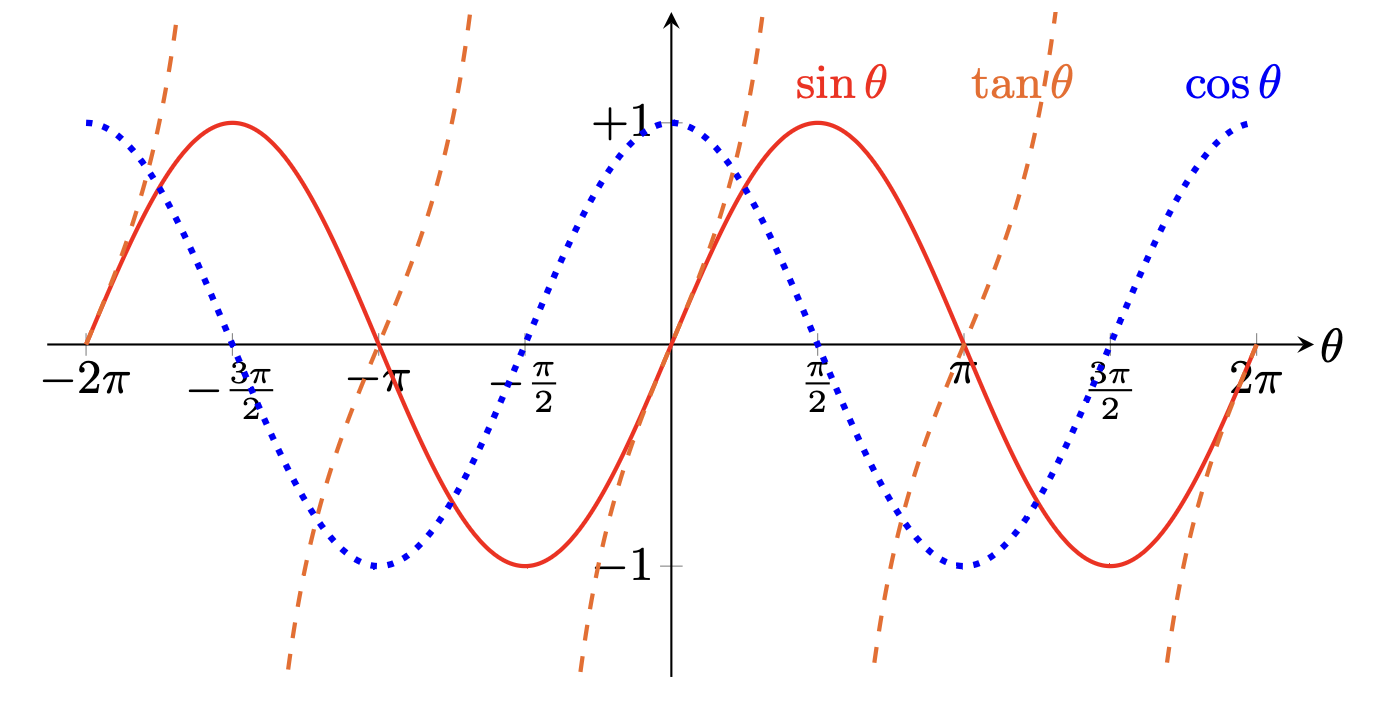
\includegraphics[width=\textwidth]{2_trig1}

\subsection{Basic Properties and Inverse Functions}

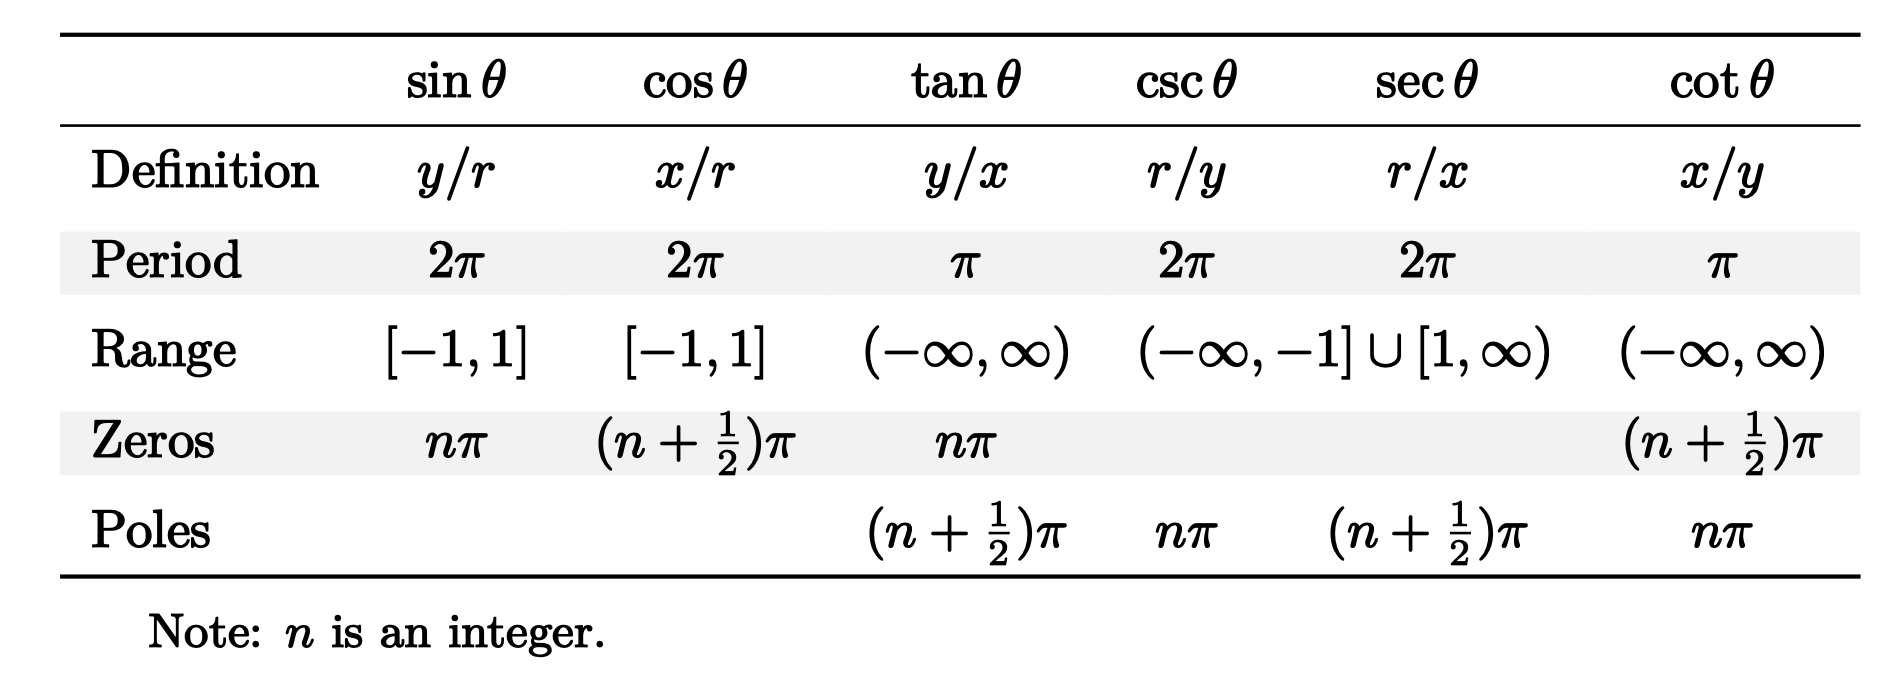
\includegraphics[width=\textwidth]{2_trig2}

% --- 1. Trig Functions ---
\begin{center}
\begin{tikzpicture}[scale=1.5]
\begin{axis}[
    axis lines=middle,
    xlabel={}, ylabel={},
    xmin=-pi, xmax=pi,
    ymin=-5, ymax=5,
    restrict y to domain=-5:5,
    samples=300,
    legend style={at={(1.05,1)}, anchor=north west},
    domain=-2*pi:2*pi
]
\addplot[blue, thick] {sin(deg(x))};
\addlegendentry{$\sin(x)$}

\addplot[red, thick] {cos(deg(x))};
\addlegendentry{$\cos(x)$}

\addplot[green!70!black, thick] {tan(deg(x))};
\addlegendentry{$\tan(x)$}

\addplot[orange, thick, domain=-2*pi:-0.1] {1/sin(deg(x))};
\addplot[orange, thick, domain=0.1:2*pi] {1/sin(deg(x))};
\addlegendentry{$\csc(x)$}

\addplot[yellow, thick, domain=-2*pi:-pi/2-0.1] {1/cos(deg(x))};
\addplot[yellow, thick, domain=-pi/2+0.1:pi/2-0.1] {1/cos(deg(x))};
\addplot[yellow, thick, domain=pi/2+0.1:2*pi] {1/cos(deg(x))};
\addlegendentry{$\sec(x)$}

\addplot[brown, thick, domain=-2*pi:-0.1] {cos(deg(x))/sin(deg(x))};
\addplot[brown, thick, domain=0.1:2*pi] {cos(deg(x))/sin(deg(x))};
\addlegendentry{$\cot(x)$}

\end{axis}
\end{tikzpicture}
\end{center}

We can also see that there are certain useful symmetric properties of the trigonometric functions

\begin{align*}
\sin(-\theta) &= - \sin(\theta)           &  \sin(\pi-\theta) &= \sin(\theta)              &  \sin(\pi+\theta) &= - \sin(\theta)\\
\cos(-\theta) &= \cos(\theta)         &  \cos(\pi-\theta) &= - \cos(\theta)   &  \cos(\pi+\theta) &= - \cos(\theta)\\
\tan(-\theta) &= - \tan(\theta)   &  \tan(\pi-\theta) &= - \tan(\theta)         &  \tan(\pi+\theta) &= \tan(\theta)
\end{align*}

There are also some common inverse functions associated with the functions.

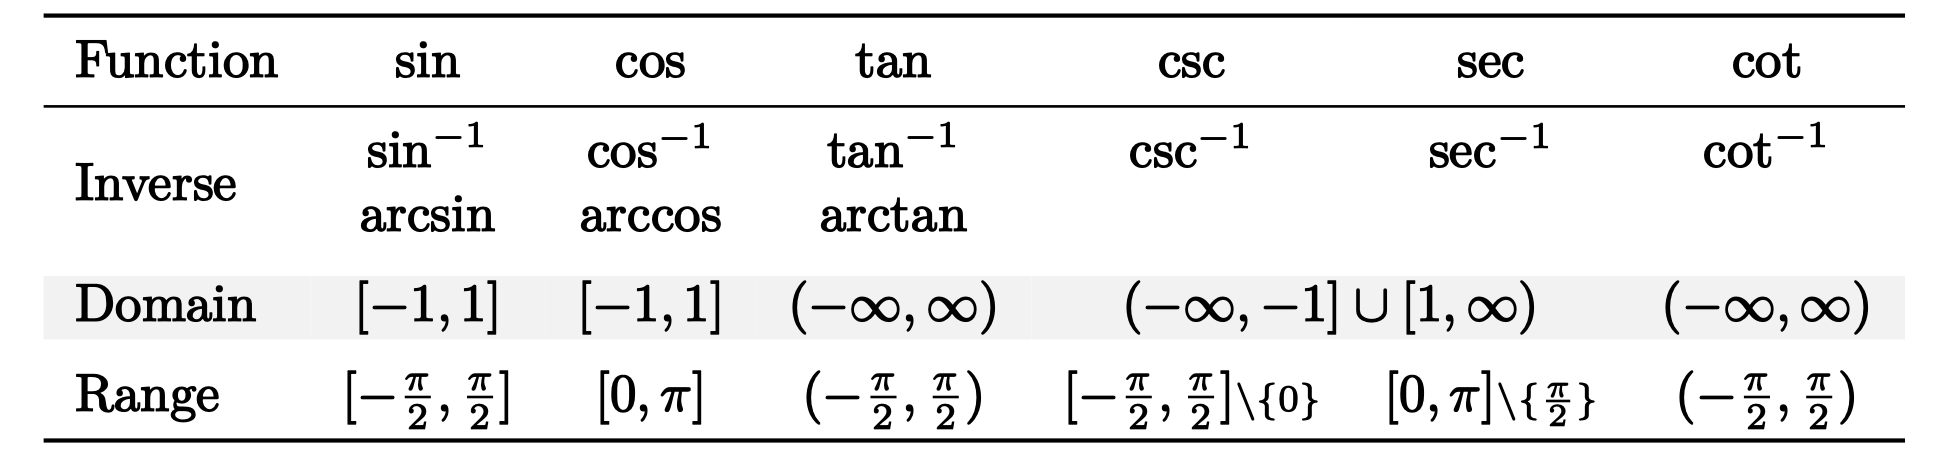
\includegraphics[width=\textwidth]{2_trig4}

But also some interesting extensions of the commonly known inverse functions, with the example being $\mathrm{arctan2}$, a function that effectively doubles the domain of the function while preserving its properties for the purpose of, say, converting values from cartesian to spherical coordinates for the azimuthal angle $\phi$.

\[
\mathrm{arctan2}(y, x) = 
\begin{cases}
  \arctan\left(\dfrac{y}{x}\right) & \text{if } x > 0, \\[2ex]
  \arctan\left(\dfrac{y}{x}\right) + \pi & \text{if } x < 0 \text{ and } y \geq 0, \\[2ex]
  \arctan\left(\dfrac{y}{x}\right) - \pi & \text{if } x < 0 \text{ and } y < 0, \\[2ex]
  +\dfrac{\pi}{2} & \text{if } x = 0 \text{ and } y > 0, \\[2ex]
  -\dfrac{\pi}{2} & \text{if } x = 0 \text{ and } y < 0, \\[2ex]
  0 & \text{if } x = 0 \text{ and } y = 0.
\end{cases}
\]

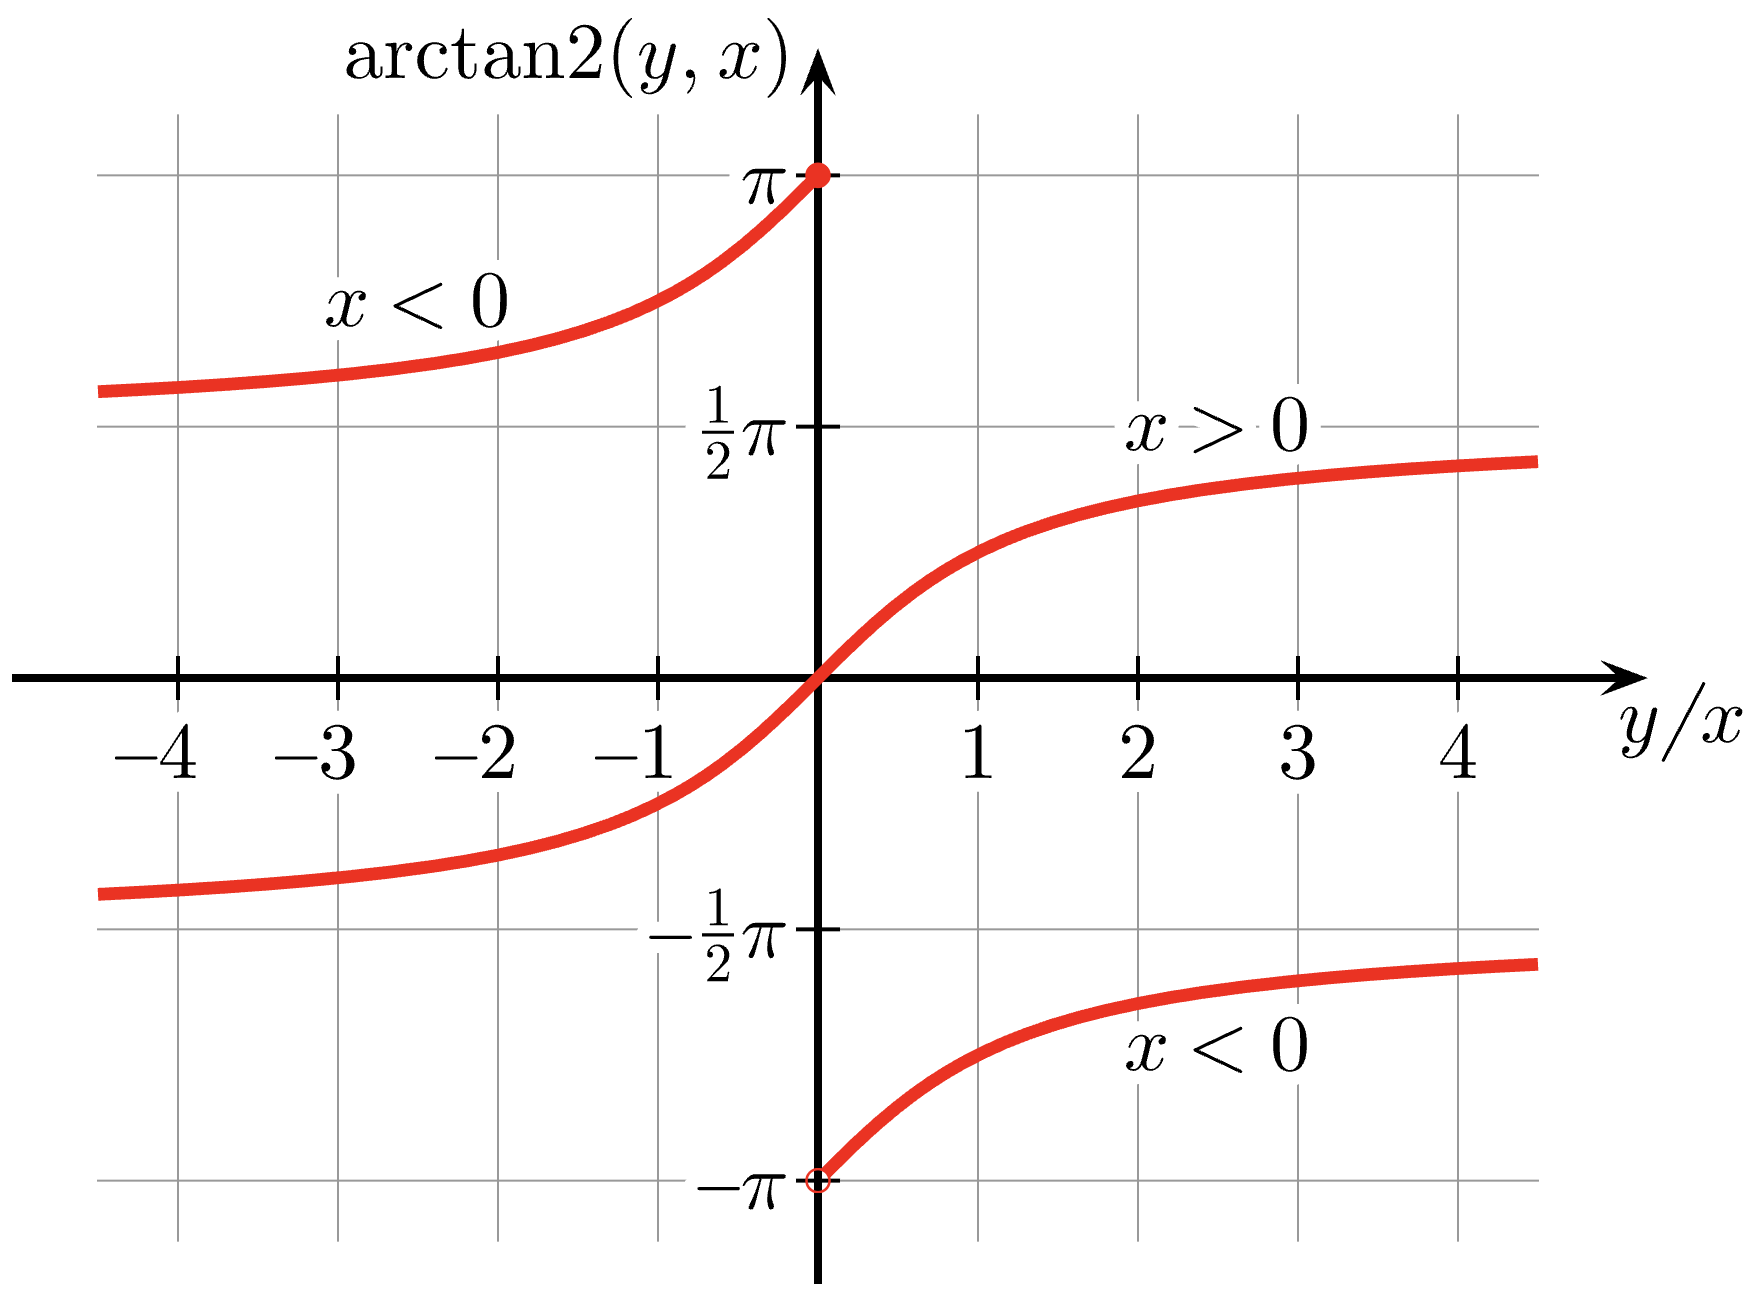
\includegraphics[width=\textwidth]{2_Arctangent2}

\subsection{Special Angles and Function Values}

There are a few special angles that are worth remembering for the trigonometric functions mentioned above, given by the wheel below.

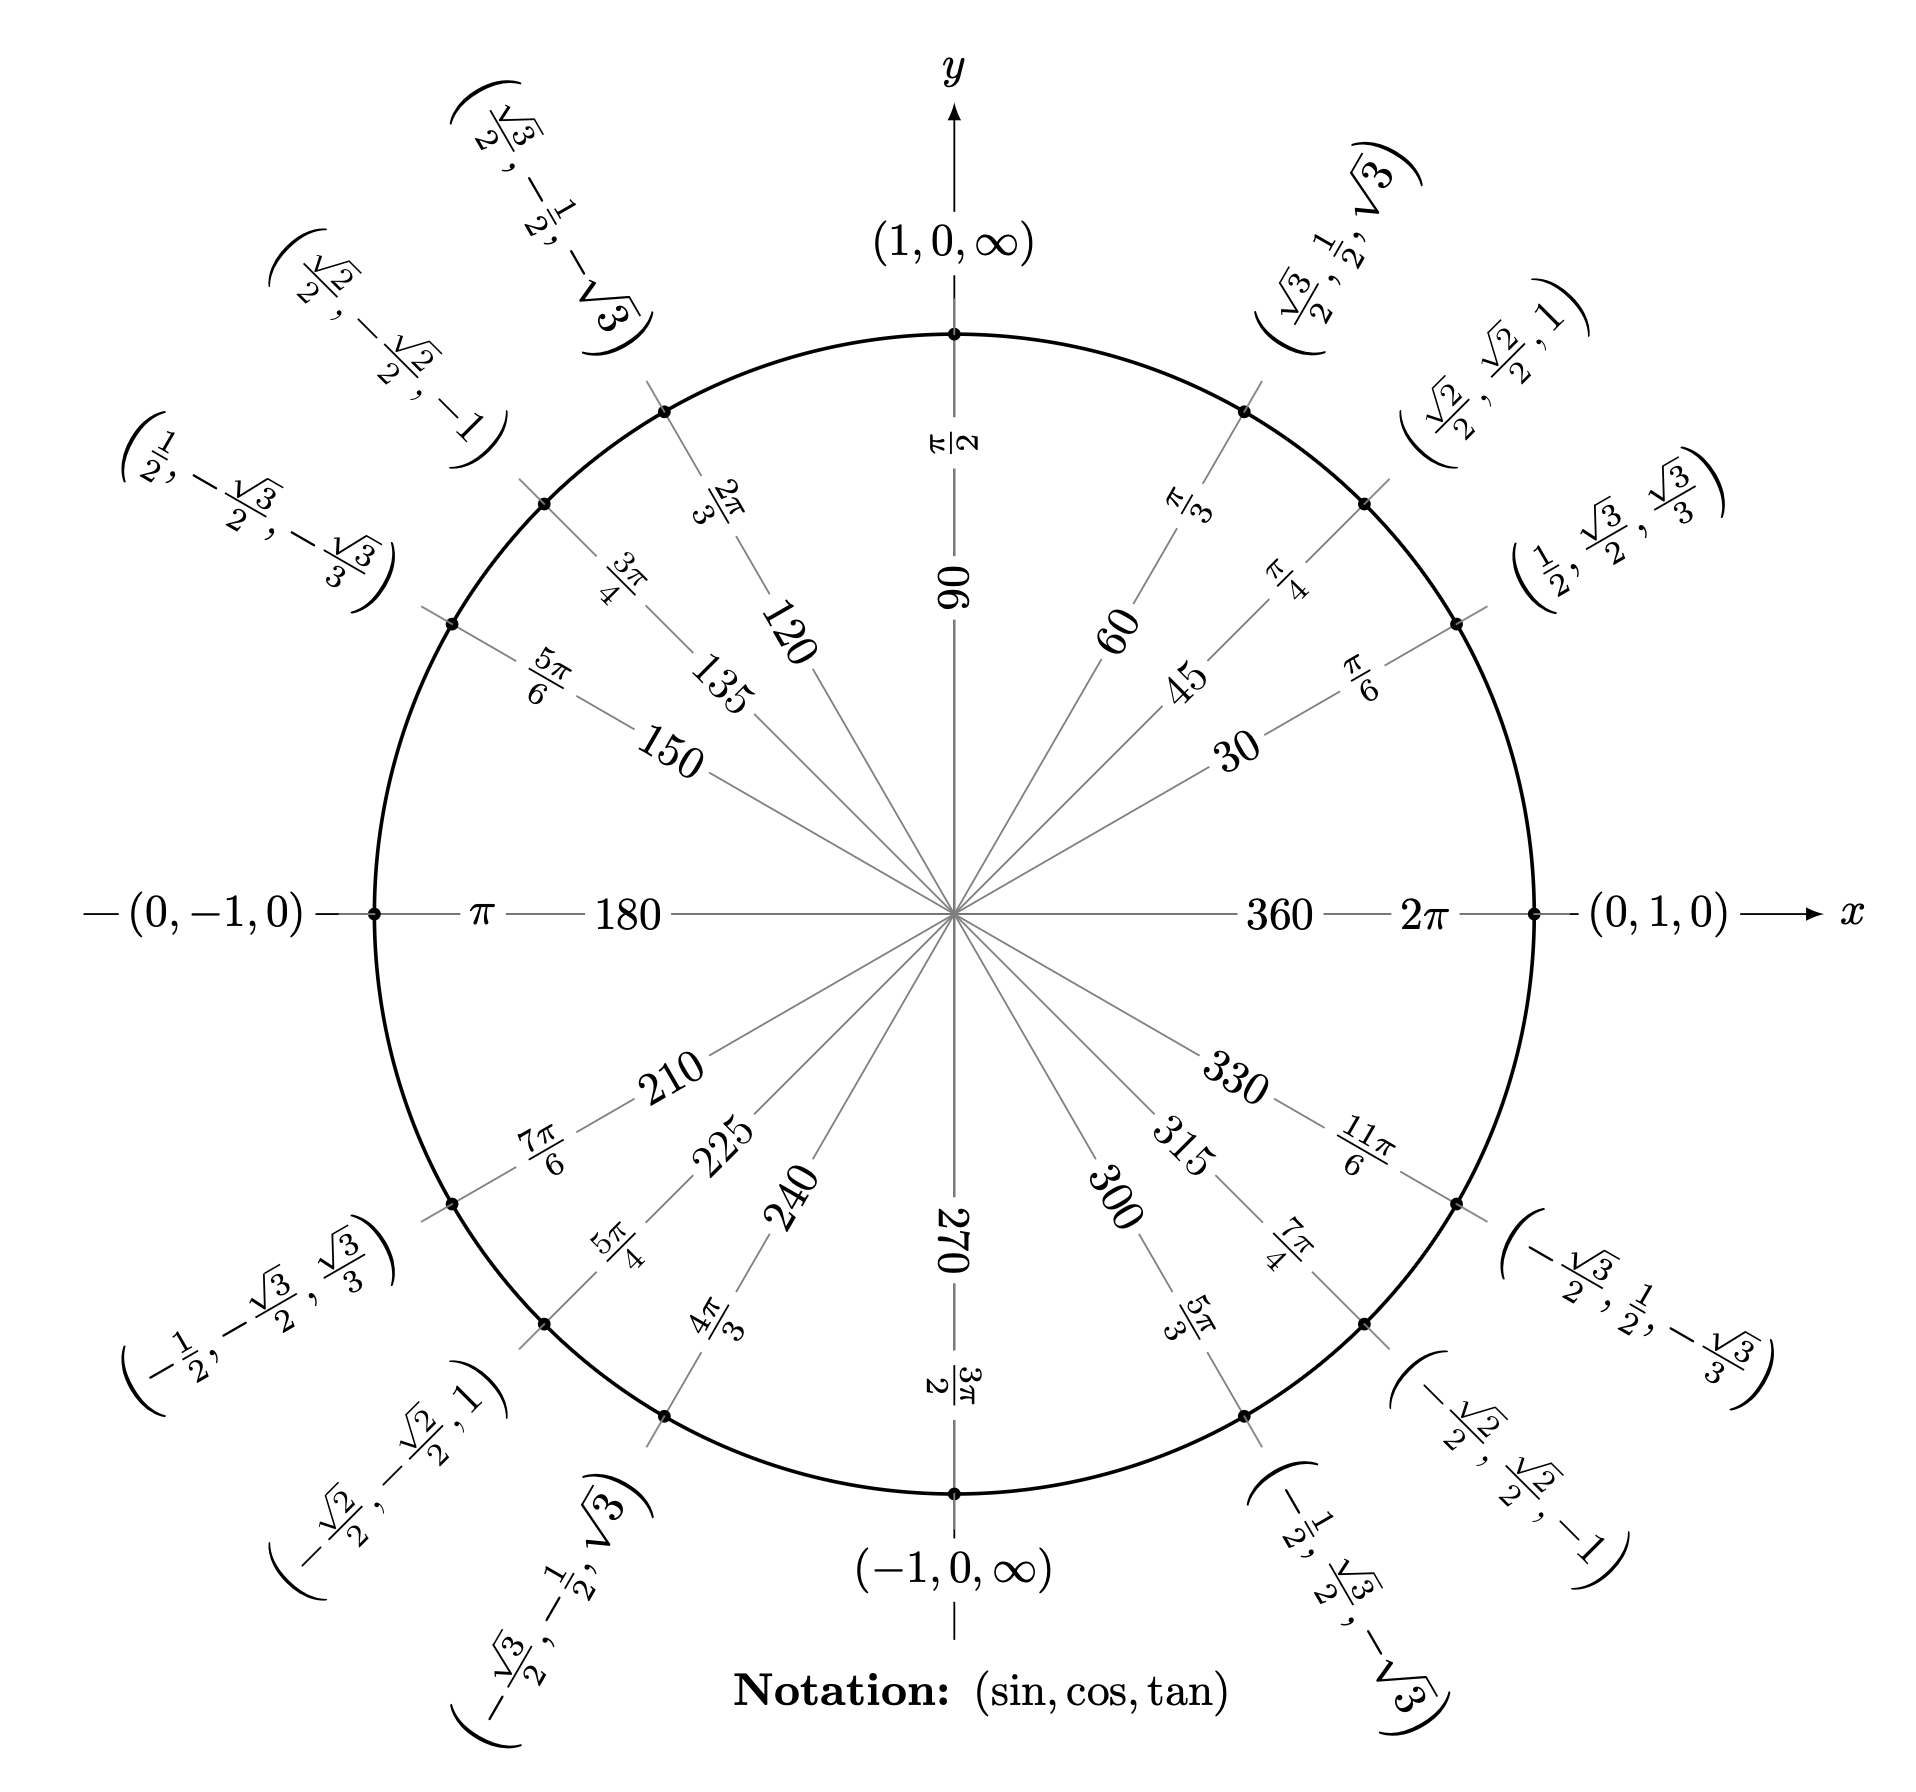
\includegraphics[width=\textwidth]{2_trig6}

\subsection{Trigonometric Identities}

\subsubsection*{Reciprocal and Quotient Identities}

\begin{align*}
\csc \theta &= \frac{1}{\sin \theta} &
\sec \theta &= \frac{1}{\cos \theta} &
\cot \theta &= \frac{1}{\tan \theta} \\
\end{align*}

\begin{align*}
    \tan \theta &= \frac{\sin \theta}{\cos \theta}, &
\cot \theta &= \frac{\cos \theta}{\sin \theta}
\end{align*}

\subsubsection*{Cofunction Identities}
\begin{align*}
\sin\!\left(\frac{\pi}{2} - \theta \right) &= \cos \theta, &
\cos\!\left(\frac{\pi}{2} - \theta \right) &= \sin \theta \\
\tan\!\left(\frac{\pi}{2} - \theta \right) &= \cot \theta, &
\cot\!\left(\frac{\pi}{2} - \theta \right) &= \tan \theta \\
\sec\!\left(\frac{\pi}{2} - \theta \right) &= \csc \theta, &
\csc\!\left(\frac{\pi}{2} - \theta \right) &= \sec \theta
\end{align*}

\subsubsection*{Pythagorean Identities}
\begin{align*}
\sin^2 \theta + \cos^2 \theta &= 1 \\
1 + \tan^2 \theta &= \sec^2 \theta \\
1 + \cot^2 \theta &= \csc^2 \theta
\end{align*}

\subsubsection*{Even–Odd Symmetry}
\begin{align*}
\sin(-\theta) &= -\sin \theta, &
\cos(-\theta) &= \cos \theta, &
\tan(-\theta) &= -\tan \theta \\
\csc(-\theta) &= -\csc \theta, &
\sec(-\theta) &= \sec \theta, &
\cot(-\theta) &= -\cot \theta
\end{align*}

\subsubsection*{Sum and Difference Formulas}
\begin{align*}
\sin(\alpha \pm \beta) &= \sin \alpha \cos \beta \pm \cos \alpha \sin \beta \\
\cos(\alpha \pm \beta) &= \cos \alpha \cos \beta \mp \sin \alpha \sin \beta \\
\tan(\alpha \pm \beta) &= \frac{\tan \alpha \pm \tan \beta}{1 \mp \tan \alpha \tan \beta}
\end{align*}

\subsubsection*{Double Angle Formulas}
\begin{align*}
\sin(2\theta) &= 2\sin \theta \cos \theta \\
\cos(2\theta) &= \cos^2 \theta - \sin^2 \theta \\
&= 2\cos^2 \theta - 1 \\
&= 1 - 2\sin^2 \theta \\
\tan(2\theta) &= \frac{2\tan \theta}{1 - \tan^2 \theta}
\end{align*}

\subsubsection*{Half Angle Formulas}
\begin{align*}
\sin^2\!\left(\frac{\theta}{2}\right) &= \frac{1 - \cos \theta}{2} \\
\cos^2\!\left(\frac{\theta}{2}\right) &= \frac{1 + \cos \theta}{2} \\
\tan\!\left(\frac{\theta}{2}\right) &= \frac{\sin \theta}{1 + \cos \theta} 
= \frac{1 - \cos \theta}{\sin \theta}
\end{align*}

\subsubsection*{Product-to-Sum Identities}
\begin{align*}
\sin \alpha \sin \beta &= \frac{1}{2}\big[\cos(\alpha - \beta) - \cos(\alpha + \beta)\big] \\
\cos \alpha \cos \beta &= \frac{1}{2}\big[\cos(\alpha - \beta) + \cos(\alpha + \beta)\big] \\
\sin \alpha \cos \beta &= \frac{1}{2}\big[\sin(\alpha + \beta) + \sin(\alpha - \beta)\big]
\end{align*}

\subsubsection*{Sum-to-Product Identities}
\begin{align*}
\sin \alpha + \sin \beta &= 2 \sin\!\left(\frac{\alpha + \beta}{2}\right) 
                           \cos\!\left(\frac{\alpha - \beta}{2}\right) \\
\sin \alpha - \sin \beta &= 2 \cos\!\left(\frac{\alpha + \beta}{2}\right) 
                           \sin\!\left(\frac{\alpha - \beta}{2}\right) \\
\cos \alpha + \cos \beta &= 2 \cos\!\left(\frac{\alpha + \beta}{2}\right) 
                           \cos\!\left(\frac{\alpha - \beta}{2}\right) \\
\cos \alpha - \cos \beta &= -2 \sin\!\left(\frac{\alpha + \beta}{2}\right) 
                           \sin\!\left(\frac{\alpha - \beta}{2}\right)
\end{align*}

A rather nice photo to sum the secion up is by relating the angles to each other using the following image

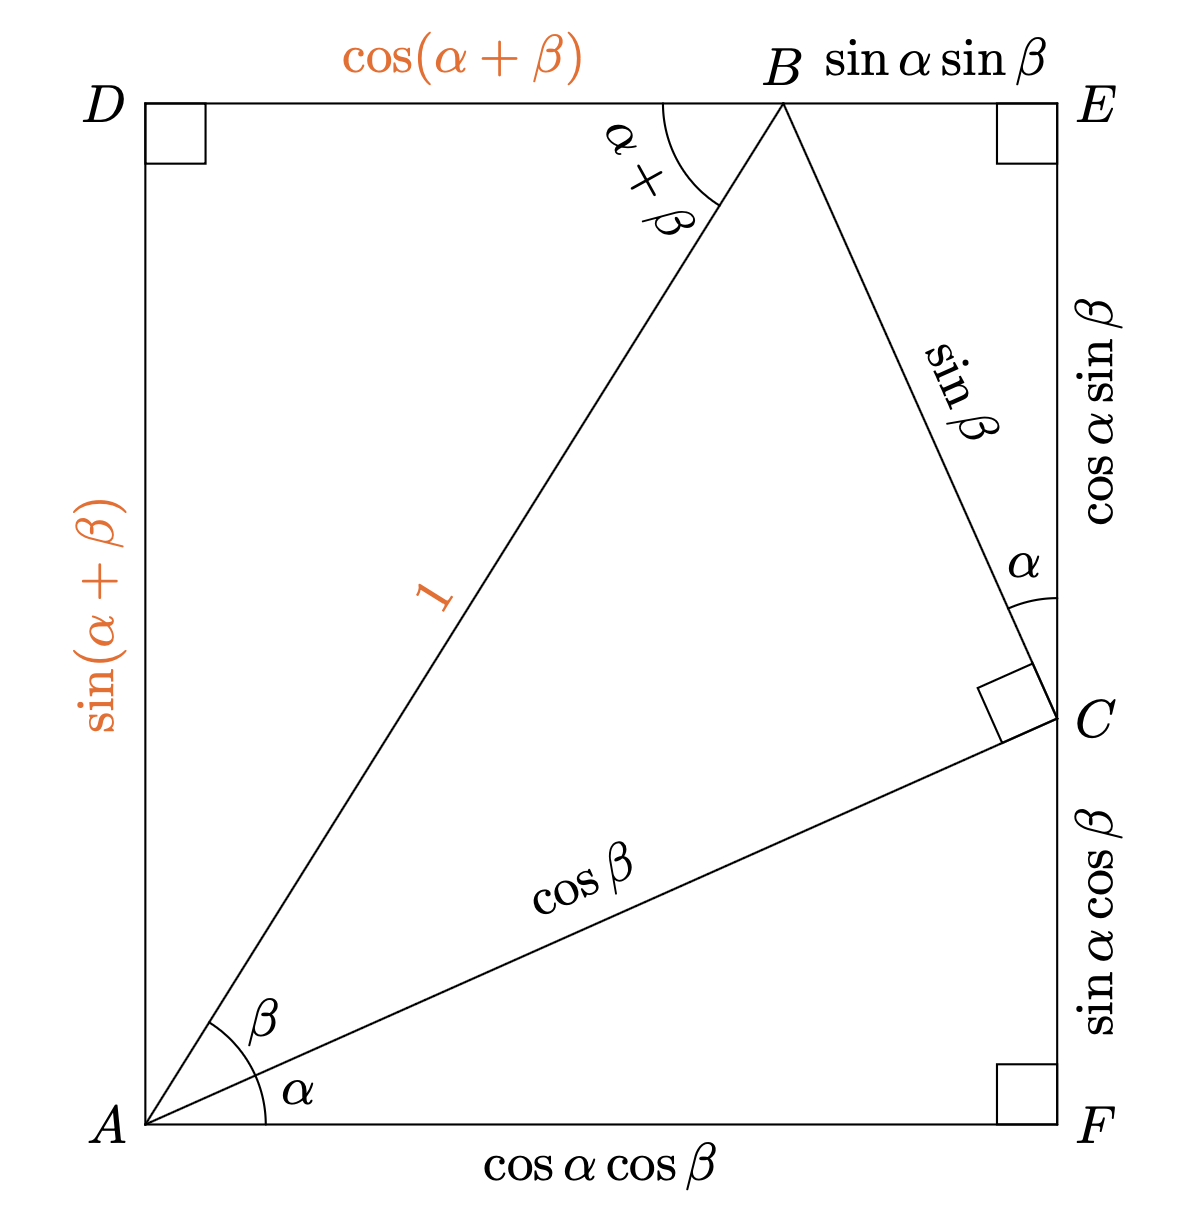
\includegraphics[width=\textwidth]{2_trig7.png}

\subsection{The Spherical Coordinate System}

While the expansion of the cartesian coordinate system into three dimensions is the logical linear expansion to take, some interesting basis begin to form if we consider the angles as a unit of measurement in three dimensions

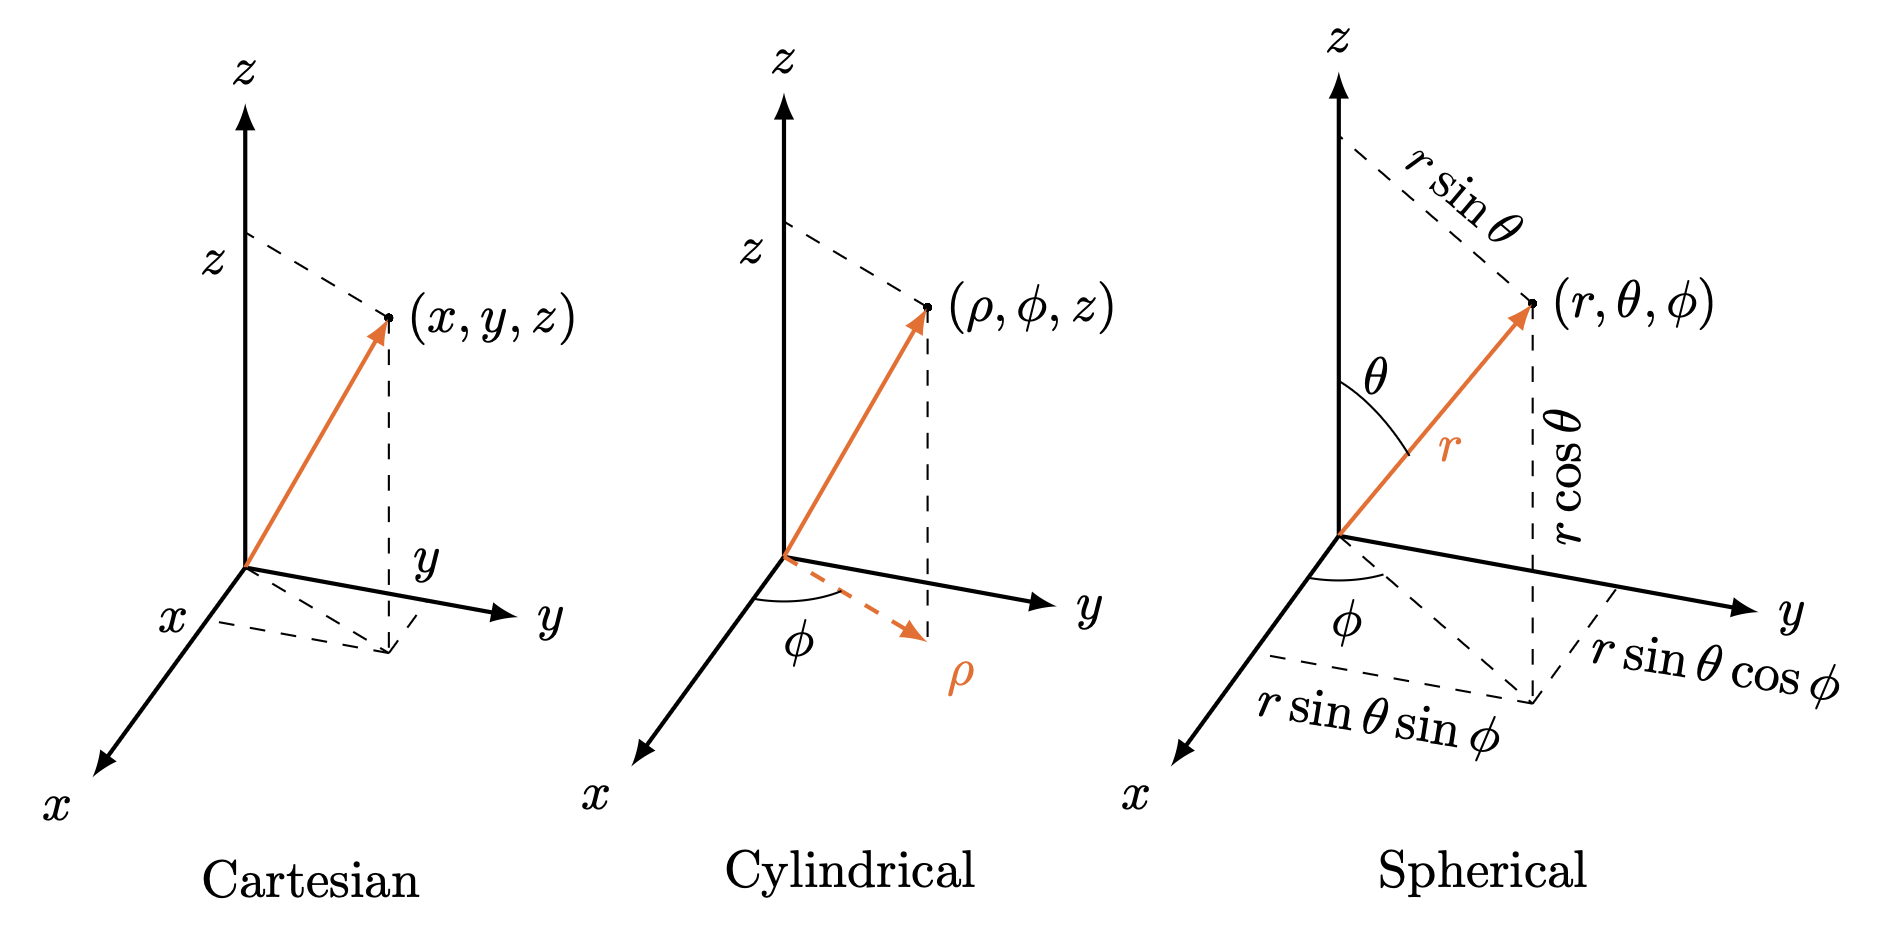
\includegraphics[width=\textwidth]{2_trig8.png}

The cylindrical coordinate system elevates the polar coordinate system into three dimensions with the addition of the $z$ axis, while the spherical system is a more organic translation of the polar coordinate system into three dimensions. While the former is best suited for describing not only cylinder-like structures yet also helices, while the latter is best suited for rotations in three-dimensional space, which is particularly potent in the field of quantum computing. 

For example, the spherical coordinate system is commonly used to represent qubit states on the Bloch sphere, employing a radius $(r)$, a polar angle $(\theta)$, and an azimuthal angle $(\phi)$ to represent a point in three-dimensional space. The azimuthal angle $\phi$ is measured in the $xy$-plane from the positive $x$-axis with common values ranging from $(-\pi, \pi]$ or $(0, 2\pi]$. The polar angle is commonly measured from the positive $z$ axis towards the $xy$-plane, with values ranging from $[0, \pi]$. Note that $r \in \mathbb{R}$, meaning that we can cover the other half of the range simply by flipping the sign around. 

Conversion is relatively simple, with conversion to and from spherical to cartesian being as follows

\begin{align*}
    x &= r \sin \theta \cos \phi &     r &= \sqrt{x^2 + y^2 + z^2} \\
    y &= r \sin \theta \sin \phi &     \phi &= \mathrm{arctan2} (y, x) \\
    z &= r \cos \theta &         \theta &= \arccos \frac{z}{r}
\end{align*}

where $\mathrm{arctan2}$ was previously defined as a optimal inverse mapping onto the range of $[- \pi, \pi]$. We also have a few definitions

\begin{definition}
    The Law of Sines is defined as 

    $$\frac{\sin A}{a} = \frac{\sin B}{b} = \frac{\sin C}{c}$$
\end{definition}

\begin{definition}
    The Law of Cosines is defined as 

    $$a^2 = b^2 + c^2 - 2bc \cos A$$

    which can be rewritten as 

    $$\cos A = \frac{b^2 + c^2 - 2bc}{a^2}$$
\end{definition}

\begin{definition}
    The Law of Tangents is defined as 

    $$\frac{a - b}{a + b} = \frac{\tan \frac{1}{2}(A - B)}{\tan \frac{1}{2}(A + B)}$$
\end{definition}


\break


\section{Complex Numbers}

We consider numbers to be complex when they compose of a real and imaginary part, and they are not only fundamental to a complete understanding of algebra and mathmatics as a whole, but also form the backbone of quantum mechanics, and, by extension, quantum computing. Mastering complex numbers is like Rosie mastering the rivet gun, so we have to study it. 

\subsection{Cartesian Form}


\begin{definition}
    A complex number $z$ is defined as 

    $$
        z = x + iy, \qquad x, y \in \mathbb{R}, \quad i^2 = -1
    $$
\end{definition}

This is called the \textbf{cartesian form} of the complex number $z$ and corresponds to a point in the two-dimensional complex plane. We commonly refer to $i$ as the imaginary unit. It may seem ironic that we need imaginary numbers in quantum computing, or that we really need the imaginary number. Take it as you may. 

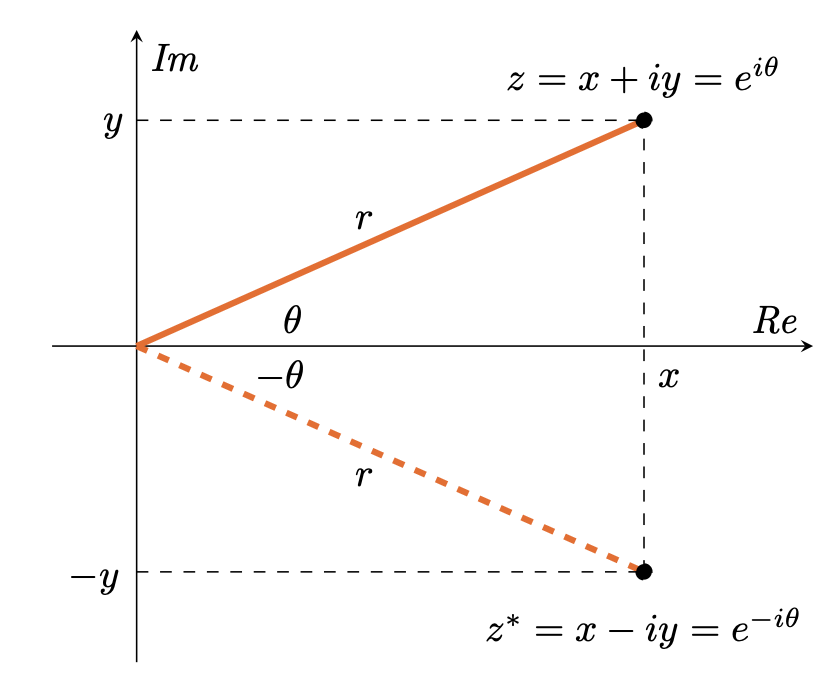
\includegraphics[width=\textwidth]{3_cn0.png}

% \[
% \begin{tikzpicture}[scale=1.2]
%   % Axes
%   \draw[->] (-0.2,0) -- (6,0) node[below right] {$\mathrm{Re}$};
%   \draw[->] (0,-3.2) -- (0,3.2) node[above left] {$\mathrm{Im}$};

%   % Points and projections
%   \coordinate (O) at (0,0);
%   \coordinate (Z) at (5,2.4);
%   \coordinate (Zc) at (5,-2.4);

%   \draw[dashed] (Z) -- (5,0) node[below] {$x$};
%   \draw[dashed] (Z) -- (0,2.4) node[left] {$y$};

%   \draw[dashed] (Zc) -- (5,0);
%   \draw[dashed] (Zc) -- (0,-2.4) node[left] {$-y$};

%   % Vectors
%   \draw[line width=1.6pt,orange] (O) -- (Z) node[midway,above right] {$r$};
%   \draw[line width=1.6pt,orange,dashed] (O) -- (Zc) node[midway,below right] {$r$};

%   % Angles
%   \draw (0.9,0) arc (0:25:0.9);
%   \node at (1.2,0.35) {$\theta$};

%   \draw (0.9,0) arc (0:-25:0.9);
%   \node at (1.3,-0.35) {$-\theta$};

%   % Dots
%   \fill (Z) circle (2pt);
%   \fill (Zc) circle (2pt);

%   % Labels near points
%   \node[above right] at (Z) {$z=x+iy=e^{i\theta}$};
%   \node[below right] at (Zc) {$z^*=x-iy=e^{-i\theta}$};
% \end{tikzpicture}
% \]


Complex numbers not motivated by quantum computing. In the numbers system, we have the real numbers $\mathbb{N}$, the integer numbers $\mathbb{Z}$, the real numbers $\mathbb{R}$, and the complex numbers $\mathbb{C}$. the set incursions go this way $\mathbb{N} \subset \mathbb{Z} \subset \mathbb{R} \subset \mathbb{C}$, all supersets of the preceeding set. The set of all complex numbers $\mathbb{C}$ is closed over all algabraic operations, which include addition, substraction, multiplication, division, power, and root, and is considered the superset of all numbers. 

\begin{definition}
    The basic components of a complex number are defined as follows. 

    $$\real(z) = x, \imaginary(z) = y$$

    which are the real and imaginary components of a complex number $z$. Of course the complex number itself has a few interesting properties, such as $i^2 = -1$, $i^3 = -i$, and $i^4 = 1$. The complex conjugate of a complex number $z$ is defined as 

    $$z^* = x - iy$$

    defined as inverting the sign of the imaginary component. We can express the modulus (vector length) and argument (angle with respect to the real axis) (which are $r$ and $\theta$ in polar coordinates), as follows:

    $$r = \vert z \vert = \sqrt{zz^*} = \sqrt{x^2 + y^2}$$

    A very convenient property derived from algebra is that $zz^* = x^2 + y^2$.

    $$\theta = arg(z)$$

    For the angle, we note that

    $$\tan \frac{y}{x} \Longrightarrow \mathrm{arctan2}(x, y)$$

    where $\mathrm{arctan2}$ has been defined in the previous section. 
\end{definition}

\begin{example}
    Given $z = 1 + \sqrt{3}i$, we have

    $$z^* = 1-\sqrt{3}\,i.$$

    $$|z|=\sqrt{1^2+(\sqrt{3})^2}=2.$$

    $$zz^*=(1+\sqrt{3}\,i)(1-\sqrt{3}\,i)=1-(\sqrt{3}\,i)^2=1+3=4=|z|^2.$$

    $$\theta=\arctan\!\left(\dfrac{\sqrt{3}}{1}\right)=\dfrac{\pi}{3}.$$

\end{example}


\subsection{Exponential Form}

Now it is worth noting that while we commonly write $z = x + iy$ to represent a complex numnber, we like to use the following definitions of the complex number in polar form to represent a complex number itself, defined as $z = r (\cos \theta + i \sin \theta)$. However, multiplication and its inverse operation, division, becomes unnecessarily difficult givne the presence of another notation, namely \textbf{exponential form}. 


\begin{definition}
    The exponential/euler forms of the complex numbers can be thought of as a circular form of the function $z = x + iy$. In polar coordinates, we can rewrite this number as 

    $$
        z = r \cos \theta + i \sin \theta, \qquad r \in \mathbb{R}
    $$
    Conversely, the conversion between cartesian and polar are 
    
    $$
    x = r \cos \theta \qquad y = r \sin \theta
    $$
    
    The formula for $z$ above can be rewritten as 

    $$z = r e^{i\theta}$$
\end{definition}


\begin{theorem}
    Euler's formula states that for any complex number $z = r \cos \theta + i \sin \theta$, we have:

    $$
    e^{i \theta} = \cos \theta + i \sin \theta
    $$
\end{theorem}

\begin{proof}
    Euler's formula can be proven using the Taylor series expansion for the functions:

    \[
    e^x = 1 + x + \frac{x^2}{2!} + \frac{x^3}{3!} + \cdots
    \]

    \[
    \sin x = x - \frac{x^3}{3!} + \frac{x^5}{5!} - \cdots
    \]

    \[
    \cos x = 1 - \frac{x^2}{2!} + \frac{x^4}{4!} - \cdots
    \]

    if we replace $x$ in the formula for $e^x$ with $e^{ix}$, we then have 

    \begin{align*}
    e^{ix} &= 1 + (ix) + \frac{(ix)^2}{2!} + \frac{(ix)^3}{3!} + \frac{(ix)^4}{4!} + \frac{(ix)^5}{5!} + \frac{(ix)^6}{6!} + \frac{(ix)^7}{7!} + \cdots \\
    &= 1 + i x - \frac{x^2}{2!} - i \frac{x^3}{3!} + \frac{x^4}{4!} + i \frac{x^5}{5!} - \frac{x^6}{6!} - i \frac{x^7}{7!} + \cdots \\
    &= \left(1 - \frac{x^2}{2!} + \frac{x^4}{4!} - \frac{x^6}{6!} + \cdots \right) + \left(i x - i \frac{x^3}{3!} + i \frac{x^5}{5!}- i \frac{x^7}{7!} + \cdots\right) \\
    &= \cos \theta + i \sin \theta
    \end{align*}

    which sums up essentially what mathmaticians call the most beautiful proof man has known. If this proof were a female robot, mathematicians would compose harmonic waves and produce digital flowers in \LaTeX to please Euler's genius. 
\end{proof}

As noted before, we know that the set of all algebraic operations is well defined and closed on the set of all complex numbers $\mathbb{C}$. Addition will be easier in cartesian form, while multiplication will be considerably simpler in exponential form. Conversion between the two is also not difficult:

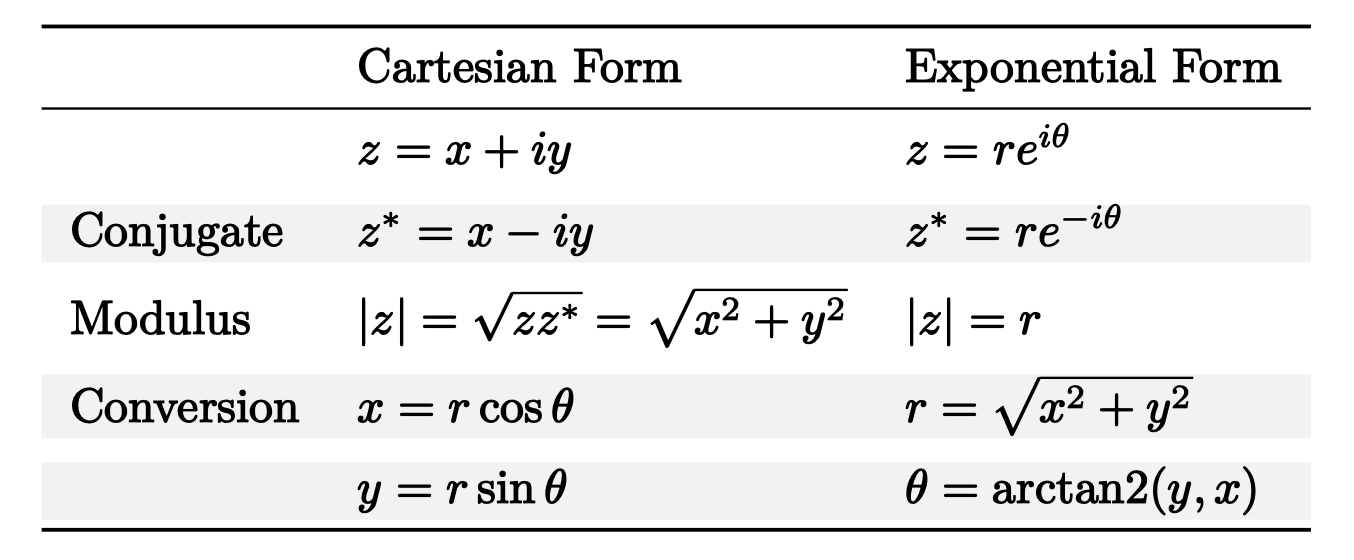
\includegraphics[width=\textwidth]{3_cn2}

% $$
% \begin{array}{l|l|l}
%  & \text{Cartesian} & \text{Exponential} \\
% \hline
% \text{} & z = x + iy & z = r e^{i\theta} \\
% \text{Conjugate} & z^{*} = x - iy & z^{*} = r e^{-i\theta} \\
% \text{Modulus} & |z| = \sqrt{x^{2}+y^{2}} & |z| = r \\
% \text{Conversion} & x = r\cos\theta,\; y = r\sin\theta & r = \sqrt{x^{2}+y^{2}},\; \theta=\operatorname{arctan2}(y,x) \\
% \end{array}
% $$


\subsection{Basic Operations}

As we touched upon earlier, the set of all complex numbers are closed on operations of addition and subtraction:

$$z_1+z_2=(x_1+x_2)+i(y_1+y_2).$$

$$z_1-z_2=(x_1-x_2)+i(y_1-y_2).$$

As well on multiplication and division. For 

$$z_1=r_1 e^{i\theta_1} \qquad z_2=r_2 e^{i\theta_2}$$ 

We have:

$$z_1\cdot z_2=r_1 r_2 e^{i(\theta_1+\theta_2)}.$$

$$\displaystyle \frac{z_1}{z_2}=\frac{r_1 e^{i\theta_1}}{r_2 e^{i\theta_2}}=\frac{r_1}{r_2}e^{i(\theta_1-\theta_2)}.$$

We also have the following properties for the conjugates of complex numbers

\begin{align*}
    \vert z \vert &= \vert z^* \vert \\
    (z_1 \pm z_2)^* &= z_1^* \pm z_2^* \\
    (z_1 \cdot z_2)^* &= z_1^* \cdot z_2^* \\
    (z_1 / z_2)^* &= z_1^* / z_2^* \\
    (z^x)^* &= (z^*)^x \quad x \in \mathbb{R}\\
    (x^z)^* &= x^{z^*} \quad x \in \mathbb{R}
\end{align*}

Where the last two are not immediately obvious. To prove that $(z^x)^* = (z^*)^x$, it is useful to write out $z$ using the complex notation $r e^{i\theta}$, and the last property is best proven using the identity $a^b = e^{b \ln a}$. As for powers and roots of complex numbers, we have 

\begin{theorem}
    De Moivre's theorem states that

    $$(\cos \theta + i \sin \theta)^s = \cos{s \theta} + i \sin{s \theta}$$

    which is conveniently derived from the fact that $z^s = r^s e^{is\theta}$.
\end{theorem}

In particular, an application of this theorem is where we describe the roots of unity. Any root of unity can be descibed by a power of the first root of unity, 

$$\omega_1 = e^\frac{2 \pi i}{n}$$

the $n$-th roots of unity ($n \in \mathbb{N}$) are given by

$$
\omega_k = e^{\frac{2\pi i}{n} k} = w_1^k \qquad k = 1, 2, \ldots, n-1
$$

which essentially says that there are $n$ roots to the complex polynomial. For $n=5$, we have the 5 roots of unity given by

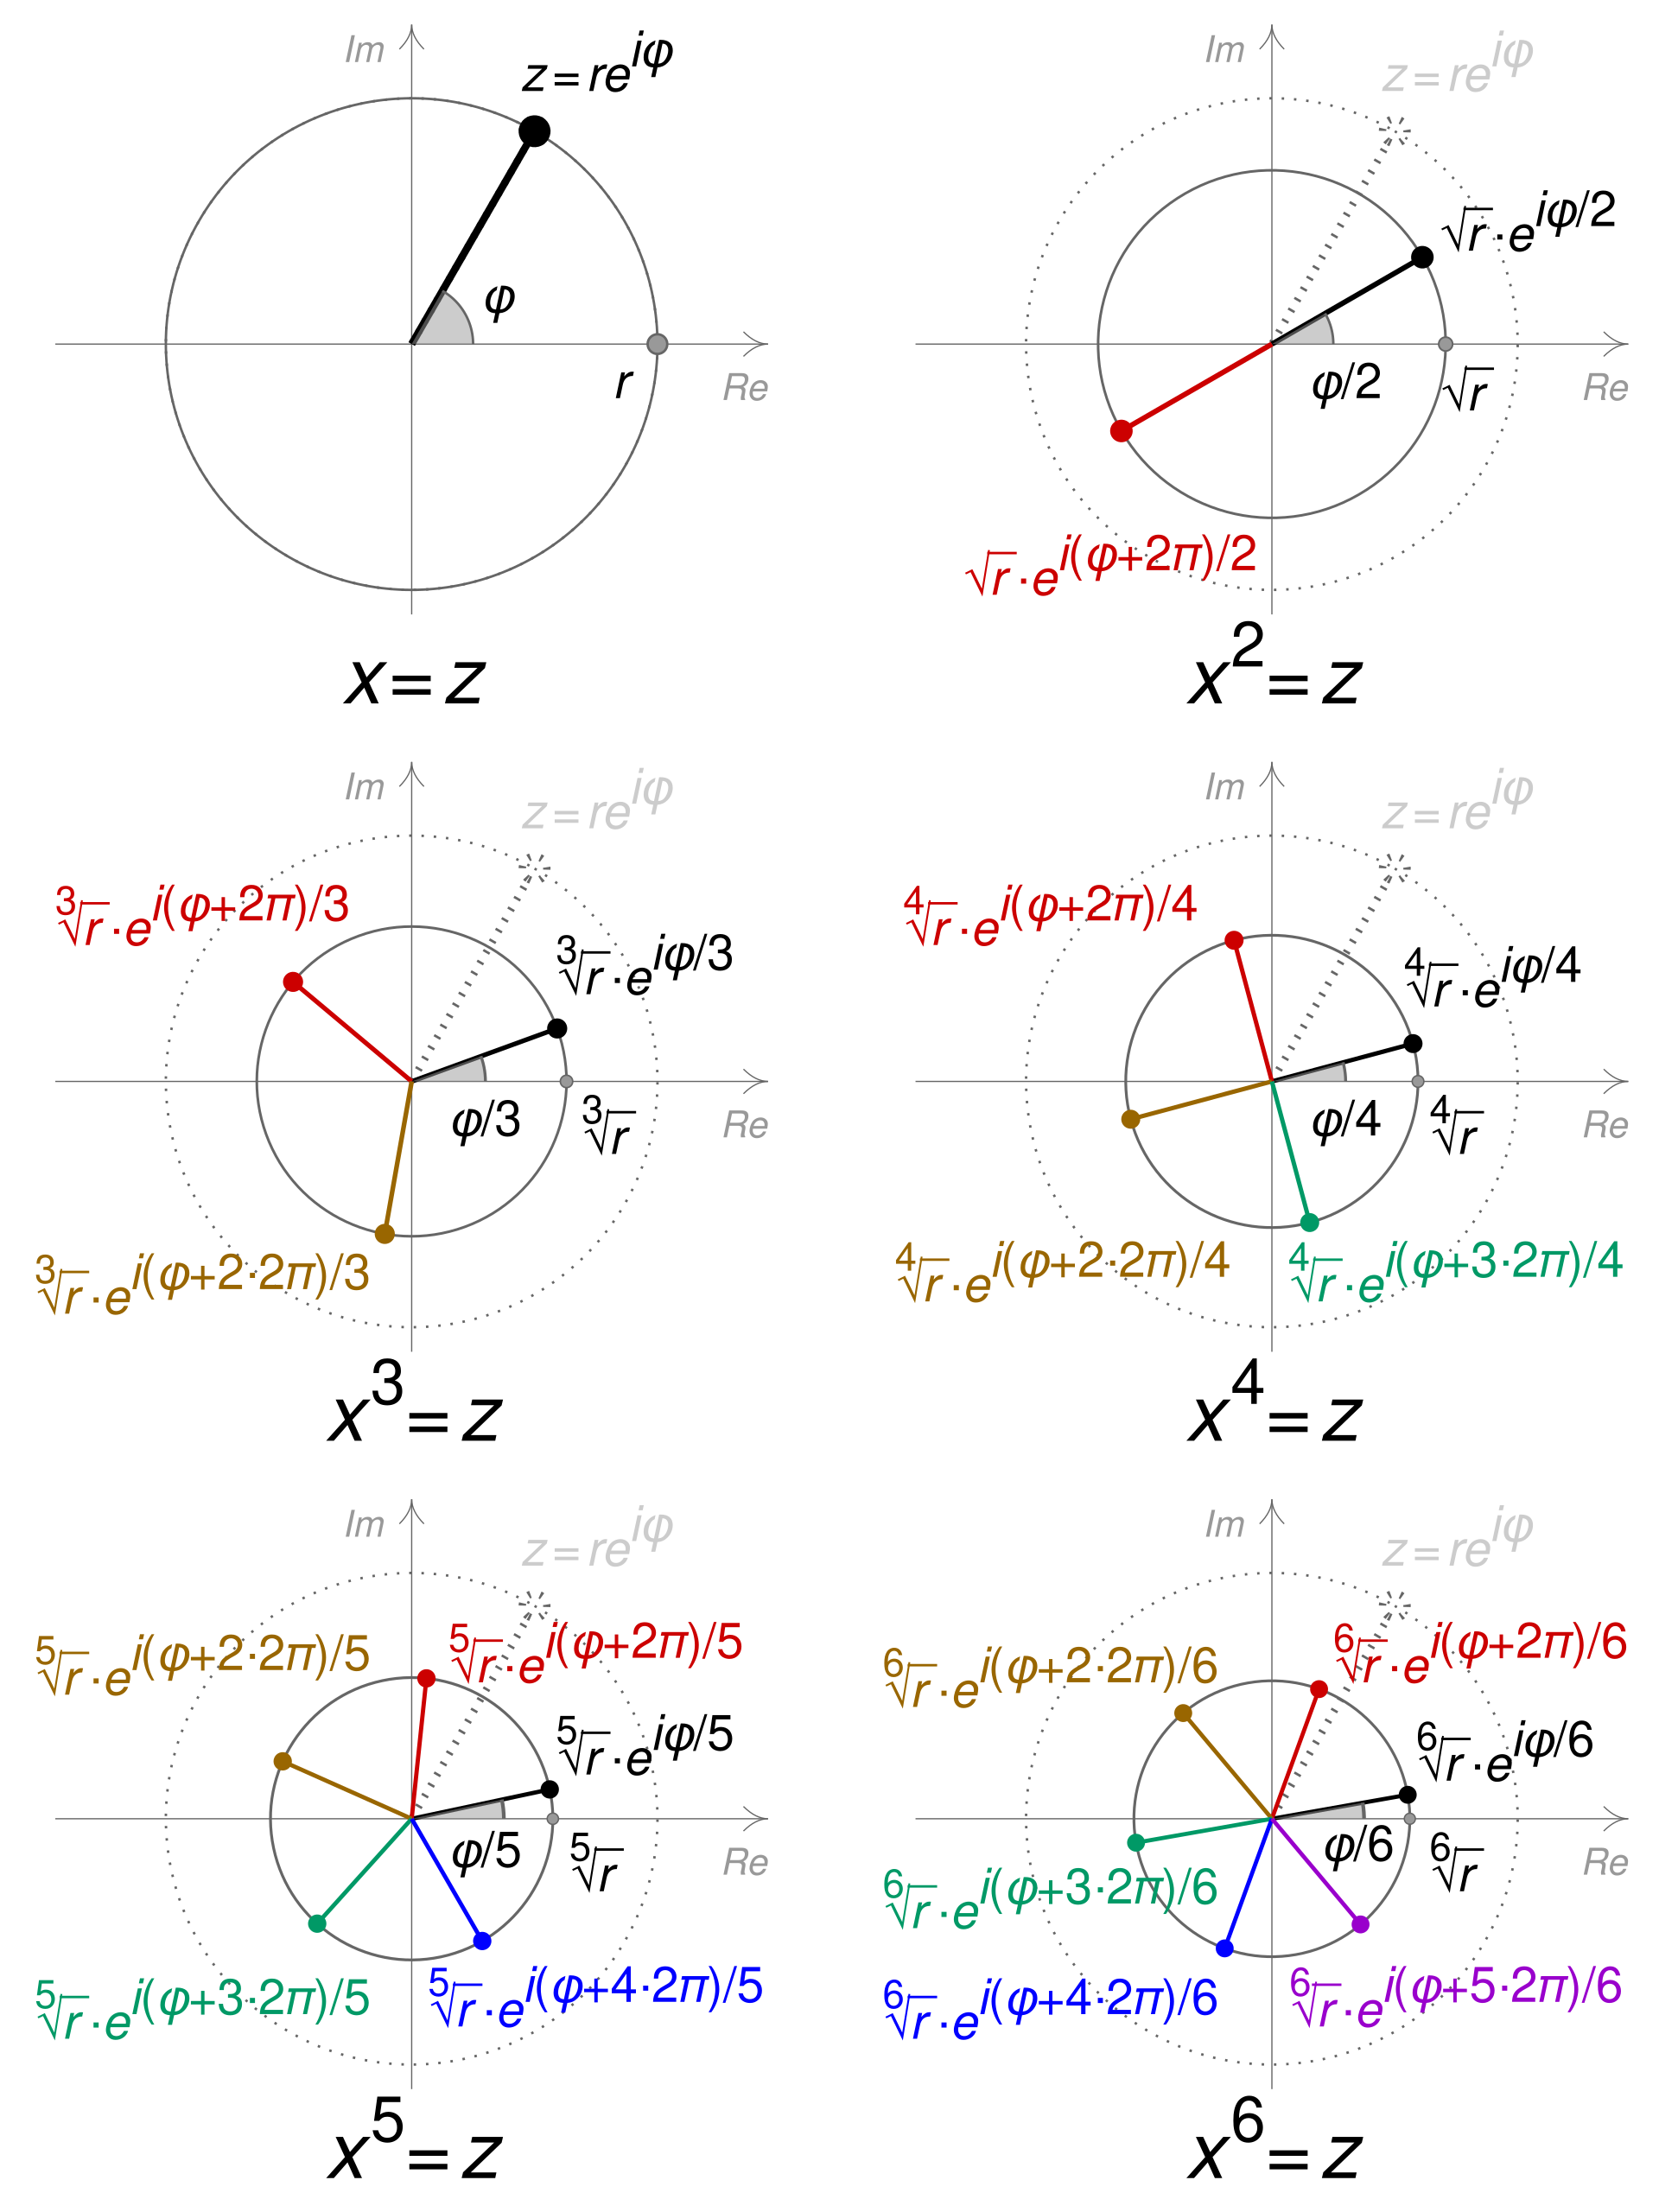
\includegraphics[width=\textwidth]{3_roots_unity}

In general, we say that there are $n$ values of $k$ that satisfy the equation $\displaystyle \omega_1^n = e^{(\frac{2 \pi i}{n})^n} = 1$. From this, we can generalize what we know into the summations over $\omega_k$, which is any $k$-th root of unity except for $\omega = 1$. 

$$\sum_{k=0}^{n-1} \omega_k = \sum_{k=0}^{n-1} \omega^k_1 = 0$$

This formula can be conviniently proven by applying the formula for summing a geometric sequence to the summation. From this, we can conviniently derive a useful mathmatical condition, being

\begin{example}
    The DFT Orthonormality condition depends on two parameters $k$ and $l$, and is stated as follows

    $$
    \frac{1}{N} \sum_{n=0}^{N-1}e^{- \frac{2 \pi i}{N}kn} e^{\frac{2 \pi i}{N} ln} = \delta_{k-l \bmod N}
    $$
\end{example}

where $\delta_{k-l} \pmod{N} = 1$ if and only if $k \equiv l \pmod{N}$, else $0$. It is saying that when $k$ is congruent to $l$, equivalent to $k - l = mN$, where the difference between $k$ and $l$ is divisible by some integer $m$. The $\delta_{k-l \bmod N}$ term is a Kronecker delta of $k \equiv l \pmod{N}$, where the result is $1$ if $k \equiv l \pmod{N}$ holds and $0$ in the case of $k \ncong l \pmod{N}$. If we define $\omega = \displaystyle  e^{i \frac{2 \pi}{N}}$ as a primitive $N$th root of unity (satisfying $\omega^N = 1$), we have the derivation

$$
\begin{aligned}
\frac{1}{N}\sum_{n=0}^{N-1} e^{-\frac{2\pi i}{N}kn}\, e^{\frac{2\pi i}{N}ln}
&= \frac{1}{N}\sum_{n=0}^{N-1} \omega^{-kn}\omega^{ln} \\
&= \frac{1}{N}\sum_{n=0}^{N-1} \omega^{n(l-k)} \\
&=
\begin{cases}
\displaystyle \frac{1}{N}\sum_{n=0}^{N-1} 1 = 1, & \text{if } l \equiv k \pmod N,\\
\displaystyle \frac{1}{N}\,\frac{1-\omega^{(l-k)N}}{1-\omega^{(l-k)}} = 0, & \text{if } l \not\equiv k \pmod N
\end{cases}
\\
&= \delta_{k-l \bmod N},
\end{aligned}
$$

where we used the fact that $\omega^{n^N} = \left(\omega^N\right)^n = 1^n = 1$ for $n \in \mathbb{N}$.

\subsection{Advanced Operations}

It's probably best to illustrate more advanced operations on complex numbers with the help of some examples

\begin{example}
    Evaluating $\sqrt{i}$ or $\sqrt{\sqrt{1}}$ gives:

    $$\sqrt{i} = \left(e^{\frac{\pi i}{2}}\right)^{\frac{1}{2}} = e^{\frac{\pi i }{4}} = \cos \frac{\pi}{4} + i \sin \frac{\pi}{4} = \frac{1}{\sqrt{2}} (1 + i)$$

    The inverse is given by

    $$\left(\frac{1}{\sqrt{2}} (1 + i)\right)^2 = \frac{1}{2}(1 + 2i + i^2) = \frac{(2i)}{2} = i$$
\end{example}


\begin{example}
    Evaluating $$ \left(\frac{1}{2}+\frac{\sqrt{3}}{2}i\right)^{50} $$ gives

    $$
    \left(\frac{1}{2}+\frac{\sqrt{3}}{2}i\right)^{50}
    =\left(e^{\frac{\pi i}{3}}\right)^{50}
    =e^{\frac{50\pi i}{3}}
    =e^{\left(16+\frac{2}{3}\right)\pi i}
    =e^{\frac{2\pi i}{3}}
    =-\frac{1}{2}+\frac{\sqrt{3}}{2}i.
    $$
\end{example}


\begin{example}
    Evaluating $$2^{3+4i}$$ gives us
    $$
    2^{3+4i}=2^3\cdot 2^{4i}=8\cdot e^{4\ln(2)\,i}
    =8\cos\!\big(4\ln 2\big)+i\,8\sin\!\big(4\ln 2\big).
    $$

\end{example}

\begin{example}
    Evaluating $$\cos(3+4i)$$
    gives us
    \begin{align*}
        \cos(3+4i) &= \frac{1}{2}\!\left(e^{i(3+4i)}+e^{-i(3+4i)}\right) \\
        &= \frac{1}{2}\!\left(e^{-4+3i}+e^{4-3i}\right) \\
        &= \frac{1}{2}e^{-4}(\cos 3+i\sin 3)+\frac{1}{2}e^{4}(\cos 3-i\sin 3) \\
        &= \frac{1}{2}(e^{-4}+e^{4})\cos 3+i\,\frac{1}{2}(e^{-4}-e^{4})\sin 3 \\     
    \end{align*}

\end{example}

\begin{example}
    If we have the equation $z^5=\frac{1}{2}+\frac{\sqrt{3}}{2}i$, solving for $z$ gives

    $$
    z_k = e^{\frac{\pi i}{15}} e^{\frac{2k\pi i}{5}}
    \quad k=0,1,2,3,4.
    $$
\end{example}

It is worth noting that there exists a way to express the trigonometric functions $\sin$ and $\cos$ as a function of euler's number. We know that 

$$
e^{i\theta} = \cos \theta + i \sin \theta \qquad e^{-i\theta} = \cos \theta - i \sin \theta
$$

from this, we can derive that 

\begin{align*}
    e^{i\theta} + e^{-i\theta} &= \cos \theta + i \sin \theta + \cos \theta - i \sin \theta \\
    e^{i\theta} + e^{-i\theta} &= \cos \theta + \cos \theta\\
    \cos \theta &= \frac{1}{2}\left(e^{i\theta} + e^{-i\theta}\right)\\
\end{align*}

and that 

\begin{align*}
    e^{i\theta} + e^{-i\theta} &= \cos \theta + i \sin \theta - (\cos \theta - i \sin \theta) \\
    e^{i\theta} - e^{-i\theta} &= i \sin \theta - \left(i \sin \theta\right)\\
    \sin \theta &= \frac{1}{2i}\left(e^{i\theta} - e^{-i\theta}\right)\\
\end{align*}

Another way of expressing this is by saying

$$
\cos x = \real(e^{i\theta}) = \frac{e^{ix} + e^{-ix}}{2}
$$
$$
\sin x = \imaginary(e^{i\theta}) = \frac{e^{ix} - e^{-ix}}{2i}
$$


One final yet very important item to rememebr throughout the curriculum is that powers for complex numbers are \textbf{rotations}.

\break

\section{Sets, Groups, and Functions}

This chapter is mainly going to fly over the various mathmatical concepts that make up the backbone of many mathmatical fields, including those relevant to quantum computing. 

\subsection{Sets}

The concepts of sets are fundamental to many areas of mathmatics. A set is a well-defined collection of distinct objects, which is also an object in its own right. 

\begin{definition}[Set]
    A set is an (unordered) collection of objects, which are said to be elements or members of the set.
\end{definition}

Let $A = \{2, 4, 6, 8\}$ be the set of even numbers less than 10. The elements of this set are 2, 4, 6, and 8. We can also write sets using set-builder notation, such as $B = \{x \mid x \text{ is a vowel in the English alphabet}\} = \{a, e, i, o, u\}$.

\vspace{12pt}


\begin{definition}[Tuple]
    A tuple (or sequence) is an ordered list of elements. 
\end{definition}

Consider the tuple $T = (3, 1, 4, 1, 5)$. This is an ordered sequence where the first element is 3, the second is 1, the third is 4, the fourth is 1, and the fifth is 5. Note that the order matters and repetition is allowed, so $(3, 1, 4, 1, 5) \neq (1, 1, 3, 4, 5)$.


\vspace{12pt}


\begin{definition}[Cardinality]
    The cardinality of a set $A$, denoted $\vert A \vert$, is the number of elements in $A$.
\end{definition}

For the set $A = \{2, 4, 6, 8\}$, the cardinality is $|A| = 4$ since there are 4 elements. For the set $B = \{x, y, z\}$, we have $|B| = 3$. The empty set has cardinality $|\emptyset| = 0$.


We can categorize sets based on their cardinality into finite, countably infinite, or uncountably infinite. A set is said to be countably infinite if it can be bijectively mapped to the set of natural numbers $\mathbb{N}$ such as the set of integers $\mathbb{Z}$, while the set is said to be uncountably infinite if there is no one-to-one to the set of natural numbers, such as the set of real numbers $\mathbb{R}$.

\begin{example}
    Finite set: $A = \{1, 2, 3, 4, 5\}$ has $|A| = 5$.
    Countably infinite set: The set of integers $\mathbb{Z} = \{\ldots, -2, -1, 0, 1, 2, \ldots\}$ can be put in one-to-one correspondence with the natural numbers $\mathbb{N}$, so $|\mathbb{Z}| = |\mathbb{N}| = \aleph_0$.
    Uncountably infinite set: The set of real numbers $\mathbb{R}$ cannot be put in one-to-one correspondence with $\mathbb{N}$, so $|\mathbb{R}| > \aleph_0$.
\end{example}



\vspace{12pt}


\begin{definition}[Subset and Superset]
    We call $B$ a subset of $A$, denoted $B \subseteq A$ if $\forall b \in B, b \in A$. In this case, $A$ is a superset of $B$, denoted $B \supseteq A$. If $B$ is a subset of $A$ but not equal to $A$, then $B$ is called a proper subset of $A$, denoted $B \subset A$.
\end{definition}


Let $A = \{1, 2, 3, 4, 5\}$ and $B = \{2, 4\}$. Then $B \subseteq A$ since every element of $B$ is also in $A$. We can also say $A \supseteq B$. Since $B \neq A$, we have $B \subset A$ (B is a proper subset of A). Additionally, $A \subseteq A$ since every set is a subset of itself.


\vspace{12pt}


\begin{definition}[Union]
    The union of two sets $A$ and $B$, denoted by $A \cup B$, is the set containing all the elements in $A$, $B$, or both. 
\end{definition}

Let $A = \{1, 3, 5, 7\}$ and $B = \{2, 3, 6, 7, 8\}$. Then $A \cup B = \{1, 2, 3, 5, 6, 7, 8\}$, which contains all elements that appear in either set A or set B (or both).



\vspace{12pt}


\begin{definition}[Intersection]
    The intersection of two sets $A$ and $B$, denoted by $A \cap B$, is the set containing all the elements in both $A$ and $B$.
\end{definition}


Using the same sets $A = \{1, 3, 5, 7\}$ and $B = \{2, 3, 6, 7, 8\}$, we have $A \cap B = \{3, 7\}$, which contains only the elements that appear in both sets.



\vspace{12pt}


\begin{corollary}[Disjoint Sets]
    Two or more sets are said to be disjoint if they have no elements in common, that is, their intersection is the empty set: $A \cap B = \emptyset$
\end{corollary}


Let $A = \{1, 3, 5\}$ and $B = \{2, 4, 6\}$. These sets are disjoint because $A \cap B = \emptyset$ - they share no common elements.



\vspace{12pt}


\begin{definition}[Difference]
    The difference of two sets $A$ and $B$, denoted by $A - B$ or $A \ B$, is the set containing all the elements in $A$ but not in $B$.
\end{definition}


Let $A = \{1, 2, 3, 4, 5\}$ and $B = \{3, 4, 6, 7\}$. Then $A - B = \{1, 2, 5\}$, which contains the elements in A that are not in B. Similarly, $B - A = \{6, 7\}$.


\vspace{12pt}



\begin{definition}[Universal Set]
    The universal set, denoted by $U$, is the set that contains all elements under consideration, usually in relation to a particular problem or discussion. Every other set in that context is a subset of the universal set $U$.
\end{definition}

In a problem about students at a university, the universal set might be $U = $ all students at the university. If we're discussing card games, the universal set could be $U = $ all 52 cards in a standard deck.



\vspace{12pt}



\begin{definition}[Complement]
    The complement of a set $A$, denoted by $\overline{A}$ or $A^{c}$, is the set of all elements in the universal set $U$ that are not in set $A$. 
\end{definition}

Let $U = \{1, 2, 3, 4, 5, 6, 7, 8, 9, 10\}$ be the universal set and $A = \{2, 4, 6, 8, 10\}$. Then the complement of A is $\overline{A} = \{1, 3, 5, 7, 9\}$, containing all elements in U that are not in A.



\vspace{12pt}


\begin{definition}[Cartesian Product]
    The cartesian product of two sets $A$ and $B$, denoted $A \cross B$, is the set of all ordered pairs $(a, b), a \in A, b \in B$. 
\end{definition}


Let $A = \{1, 2\}$ and $B = \{x, y, z\}$. Then $A \times B = \{(1,x), (1,y), (1,z), (2,x), (2,y), (2,z)\}$. The Cartesian product contains all possible ordered pairs where the first element comes from A and the second from B. Note that $|A \times B| = |A| \cdot |B| = 2 \cdot 3 = 6$.



\vspace{12pt}


\begin{definition}[Set Partitions]
    A partition of a set $A$ is a collection of disjoint subsets of $A$ such that every element in $A$ is included in exactly one subset. These subsets are called blocks of the partition. 
\end{definition}

Let $A = \{1, 2, 3, 4, 5, 6\}$. One partition of A could be $\{A_1, A_2, A_3\}$ where $A_1 = \{1, 2\}$, $A_2 = \{3, 5\}$, and $A_3 = \{4, 6\}$. These subsets are disjoint ($A_i \cap A_j = \emptyset$ for $i \neq j$) and their union gives the original set ($A_1 \cup A_2 \cup A_3 = A$).




\vspace{12pt}

\begin{theorem}[Set Partition]
    If $\{A_1, A_2, \ldots, A_n\}$ is a partition of set $A$, and $B \subseteq A$, then  $\{A_1 \cap B, A_2 \cap B, \ldots, A_n \cap B\}$ is a partition of set $B$.
\end{theorem}

Let $A = \{1, 2, 3, 4, 5, 6\}$ with partition $\{A_1, A_2, A_3\}$ where $A_1 = \{1, 2\}$, $A_2 = \{3, 5\}$, and $A_3 = \{4, 6\}$. If $B = \{2, 3, 4, 5\} \subseteq A$, then $\{A_1 \cap B, A_2 \cap B, A_3 \cap B\} = \{\{2\}, \{3, 5\}, \{4\}\}$ forms a partition of B.





\begin{definition}[Power Set]
    The power set of $A$ is the set of all subsets of $A$, denoted by $\mathcal{P}(A)$ is the set of all subsets of $A$.
\end{definition}


Let $A = \{1, 2\}$. The power set $\mathcal{P}(A)$ contains all possible subsets of A:
$\mathcal{P}(A) = \{\emptyset, \{1\}, \{2\}, \{1, 2\}\}$
Note that $|\mathcal{P}(A)| = 2^{|A|} = 2^2 = 4$. For any set with n elements, its power set has $2^n$ elements. For set operations in general, there are a few laws worth noting.

Identity Laws:
$$
A \cup \varnothing = A$$$$ A \cap U = A.
$$

Domination Laws:

$$
A \cup U = U$$$$ A \cap \varnothing = \varnothing.
$$

Idempotent Laws:
$$
A \cup A = A$$$$ A \cap A = A.
$$

Absorption Laws:
$$
A \cup (A \cap B) = A$$$$ A \cap (A \cup B) = A.
$$

Complement Laws:
$$
A \cup \overline{A} = U$$$$ A \cap \overline{A} = \varnothing$$$$ \overline{\overline{A}} = A.
$$

Commutative Laws:
$$
A \cup B = B \cup A$$$$ A \cap B = B \cap A.
$$

Associative Laws:
$$
A \cup (B \cup C) = (A \cup B)\cup C$$$$ A \cap (B \cap C) = (A \cap B)\cap C.
$$

Distributive Laws:
$$
A \cup (B \cap C) = (A \cup B)\cap (A \cup C)$$$$
A \cap (B \cup C) = (A \cap B)\cup (A \cap C).
$$

De Morgan's Laws:
$$
\overline{A \cap B}=\overline{A}\,\cup\,\overline{B}$$$$
\overline{A \cup B}=\overline{A}\,\cap\,\overline{B}.
$$


\begin{definition}[Totally Ordered Set]
A totally ordered set is a set in which every pair of elements is comparable; for any two elements $a$ and $b$, either $a \le b$ or $b \le a$ holds. 
\end{definition}

Examples include the real numbers and the integers with their usual orders.

\vspace{12pt}


\begin{definition}[Partially Ordered Set (Poset)]
A partially ordered set (poset) is a set equipped with a relation $\le$ that is reflexive, antisymmetric, and transitive; in a poset, not every pair of elements must be comparable, so some pairs may be incomparable. For example, the power set $\mathcal{P}(\mathbb{Z})$ ordered by inclusion $(\subseteq)$ contains subsets such as $\{1,2\}$ and $\{2,3\}$ that are not comparable, and the positive integers ordered by divisibility have incomparable primes like $5$ and $7$.
\end{definition}
\vspace{12pt}


\begin{definition}[Supremum]
Let $S$ be a nonempty subset of a partially ordered set $P$. An element $u \in P$ is the supremum of $S$, denoted by $u=\sup S$, if:
\begin{enumerate}
\item \textbf{Upper bound:} every $s\in S$ satisfies $s \le u$.
\item \textbf{Least upper bound:} if $v$ is any upper bound of $S$, then $u \le v$.
\end{enumerate}
For instance, $\sup\{-1,-2,-3,\dots\}=-1$, and $\sup\{\sin x: x\in[0,\pi]\}=1$.
\end{definition}
\vspace{12pt}

\begin{definition}[Infimum]
Let $S$ be a nonempty subset of a partially ordered set $P$. An element $\ell \in P$ is the infimum of $S$, denoted by $\ell=\inf S$, if:
\begin{enumerate}
\item \textbf{Lower bound:} every $s\in S$ satisfies $\ell \le s$.
\item \textbf{Greatest lower bound:} if $v$ is any lower bound of $S$, then $v \le \ell$.
\end{enumerate}
For example, $\inf\{e^{-x}: x>0\}=0$, even though $0$ is not an element of the set.
\end{definition}


\subsection{Groups}

Groups, rings, and fields lay the foundation in mathmatics that build upon sets with additional operations in algebra. These strucutres are ubiquitous in mathmatics and physics and lay the foundation for quantum computing as well. 

A group is a set equipped with a single binary operation that exhibits certain properties, much like addition and multiplication. A ring expands on this by incorporating two operations, typically referred to as multiplication and addition. A field is a more stringent structure where the set is a group under both operations, with multiplication also being commutative, and every non-zero element having a multiplicative inverse. 

\begin{definition}
    A group is a set $G$ which is \textit{closed} under an operation $\cdot$ (that is $\forall x, y \in G, x \cdot y \in G$) and satisfies the following properties:

    \begin{enumerate}
        \item \textbf{Identity:} $\exists e \in G$ where $\forall x \in G, x \cdot e = x = e \cdot x$. We define $e$ to be the identity element.
        \item \textbf{Inverse:} $\forall x \in G, \exists y \in G$ such that $x \cdot y = e = y \cdot x$, where $e$ is the identity element identified above. 
        \item \textbf{Associativity:} The operation $\cdot$ is associative for every $x, y, z \in G$, i.e. $$x\cdot(y\cdot z) = (x \cdot y)\cdot z$$
    \end{enumerate}
\end{definition}

In mathmatical contexts, it is common to omit the symbol $\cdot$ or $*$ for the group operation and simply write $x \cdot y$ as $xy$. Some common exmaples include the gorup of integers $\mathbb{Z}$ under addition, denoted by $(\mathbb{Z}, +)$, with $e = 0$, and the inverse of $x$ being $-x$. Another example would be the group of integers modulo $n$, denoted $\mathbb{Z}/n\mathbb{Z}$, with closure (the sum of any two integers modulo $n$ also forming a group under modulo $n$), identity, inverse, and associativity all holding under the subspace of $\mathbb{Z}/n\mathbb{Z}$.

\begin{definition}[Abelian Group]
   A group is said to be \textit{abelian} if the operation $\cdot$ is commutative $\forall x, y \in G$, that is, $$x \cdot y = y \cdot x$$ 
\end{definition}


While the examples so fare are all abelian groups, there are some of groups that are not abelian. For exmaple, the set of all symmetries of an equilateral triangle, known as the dihedral group $D_3$ is not abelian. As you can see, the table of operations is not symmetrical, rendering the group as a non-abelian group. However, the identity, inverse, and associative elements/properties are all present upon verification. 


\[
\begin{array}{c|cccccc}
   & e & a & b & c & r & s \\
\hline
e & e & a & b & c & r & s \\
a & a & e & r & s & b & c \\
b & b & s & e & r & c & a \\
c & c & r & s & e & a & b \\
r & r & c & a & b & s & e \\
s & s & b & c & a & e & r \\
\end{array}
\]



However, in the context of quantum computing, there are a few symmetry groups worth noting. They are

\begin{enumerate}
    \item $\mathbf{SO}(N):$ The orthogonal group in $N$ dimensions consists of all $N \cross N$ orthogonal matrices with determinant $1$, representing rotations in $\mathbb{R}^N$. These rotations preserver distance sand the orientation of objects in question. SO($2$) corresponds to a circle, and SO($3$) to a sphere. 
    \item $\mathbf{SU}(2):$ The special unitary group of degree 2 comprises of all $2 \cross 2$ unitary matrices with determinant $1$. It is closely related to SO($3$) and is commonly used to describe spins and qubit states. Each rotation in SO($3$) corresponds to two points in SU($2$). 
    \item $\mathbf{SU}(N):$ This represents the special unitary group of degree $N$, extending the concepts of SU($2$). These groups are useful in the study of quantum entanglement in quantum computing concerning $N$-level quantum systems. 
\end{enumerate}

\begin{definition}[Subgroups]
    A subgroup $H$ of group $G$ is a subset of $G$ that is a group in by itself, with the same group operation in $G$. You can think of this as a reduced version of $G$ where still 
    \begin{enumerate}
        \item The identity element of $G$ is in $H$.
        \item $\forall h_1, h_2 \in H, \quad h_1 \cdot h_2 \in H$.
        \item $\forall h \in H, \quad h^{-1} \in H$
    \end{enumerate}
\end{definition}

\begin{theorem}[Lagrange's Theorem]
    For any finite group $G$ and any subgroup $H$ of $G$, the order of $H$ divides the order of $G$, i.e. $$\vert G \vert \equiv 0 \mod \vert H \vert$$
\end{theorem}
\vspace{12pt}


\begin{definition}[Coset]
    Given a group $G$ and a subgroup $H$ of $G$, the \textbf{left coset} of $H$ with representative $g \in G$ is the set $gH = \{gh \vert h \in H\}$. Similarly, the right coset is $Hg = \{hg \vert h \in H\}$.
\end{definition}

\begin{theorem}[Parition Theorem for Cosets]
    The collection of all left cosets of a subgroup $H$ forms a partition of the group $G$. This means 
    \begin{enumerate}
        \item Every element of $G$ belongs to exactly one coset of $H$.
        \item Cosets are disjoint and have no elements in common.
    \end{enumerate}
\end{theorem}

\begin{definition}[Normal Subgroup]
    A subgroup $N$ of a group $G$ is called a normal subgroup if it is invariant under conjugation by elements of $G$. This means that $\forall n \in N, \quad g \in G, \quad gng^{-1} \in N$. In notation, $N \triangleleft G$ if $$gNg^{-1} = \{gng^{-1} \vert n \in N\} \subseteq N \forall g \in G.$$
\end{definition}

Now, note that this is not the same as an abelian group. While the abelian group imples that every subgroup is a normal subgroup, the latter does not imply the former.

\begin{example}[Quaternion Group $Q_8$]
Let $$Q_8=\{\pm 1,\pm i,\pm j,\pm k\}$$ with relations $$i^2=j^2=k^2=ijk=-1.$$ This group is non-abelian since, for instance, $ij=k$ while $ji=-k$, so $ij\neq ji$. Nevertheless, every subgroup of $Q_8$ is normal; the subgroups are $\{1\}$, $\{\pm 1\}$, $\langle i\rangle=\{\pm 1,\pm i\}$, $\langle j\rangle=\{\pm 1,\pm j\}$, $\langle k\rangle=\{\pm 1,\pm k\}$, and $Q_8$ itself, and each is invariant under conjugation by any element of $Q_8$. Thus $Q_8$ is a non-abelian group in which all subgroups are normal (a Hamiltonian group).
\end{example}



Also, it is worth noting that the left and right cosets of a normal subgroup $N$ are the same, allowing the group operations on cosets to be well-defined, which brings us to quotient groups:

\begin{definition}[Quotient Group]
    Let $G$ be a group, and $N \triangleleft G$. The quotient group $G / N$ is the set of cosets of $N \in G$ with the group operations defined by: $$(gN) (hN) (gh)N \quad \forall g, h \in G$$
\end{definition}

\begin{example}
    Consider the group $\mathbb{Z}$ of integers under addition and the subgroup $2\mathbb{Z}$ consisting of all even integers. The quotient group $\mathbb{Z}/2\mathbb{Z}$ is the set of cosets of $2\mathbb{Z}$ in $\mathbb{Z}$:

\begin{itemize}
\item The coset $0+2\mathbb{Z}=\{\ldots,-4,-2,0,2,4,\ldots\}$ represents the even integers.
\item The coset $1+2\mathbb{Z}=\{\ldots,-3,-1,1,3,5,\ldots\}$ represents the odd integers.
\end{itemize}

Thus, $\mathbb{Z}/2\mathbb{Z}$ has two elements: $0+2\mathbb{Z}$ and $1+2\mathbb{Z}$, corresponding to the even and odd integers, respectively. The group operation is addition modulo $2$.
\end{example}

This quotient group is \emph{isomorphic} to $\mathbb{Z}_2=\{0,1\}$ under addition modulo $2$, denoted as $\mathbb{Z}/2\mathbb{Z}\cong \mathbb{Z}_2$. Two groups are isomorphic if they have the same structure, meaning there is a one-to-one correspondence between the elements of the two groups that preserves the group operation.

\begin{definition}[Cyclic Group]
    A group $G$ is cyclic if $\exists g \in G$ such that $\forall x \in G$, $x$ can be expressed as powers (repeated operations) of $g$. 
\end{definition}

A good example of this would be $D_3$, which also has multiple generators. 
\vspace{12pt}

\begin{definition}[Ring]
    A ring is a set $R$ equipped with two operations $+$ and $\times$ satisfying the following properties:
    \begin{enumerate}
        \item $(R, +)$ forms an abelian group. 
        \item $(R, \times)$ is associative, that is $\forall a, b, c \in R$, $$a \times (b \times c) = (a \times b) \times c$$ 
        \item The distributive properties hold, that is $\forall a, b, c \in R$, $$a \times (b + c) = (a \times b) + (a \times c) $$$$ (b + c) \times a = (b \times a) + (c \times a)$$
    \end{enumerate}
\end{definition}

For example, both the set of integers $\mathbb{Z}$ and the group of integers modulo $n$, $\mathbb{Z}/n\mathbb{Z}$, are both rings. However, multiplication notably does not have an inverse under most groups of integers. For this to hold, we need to have fields. 

\begin{definition}[Field]
    A field is a set $F$ with two operations $+$ and $\times$, where
    \begin{enumerate}
        \item $(R, +)$ forms an abelian group. 
        \item $(R - \{0\}, \times)$ forms an abelian group. 
        \item The distributive properties holds as in rings. 
    \end{enumerate}
\end{definition}

Some common examples include the set of rational numbers $\mathbb{Q}$, the set of real numbers $\mathbb{R}$, and the set of complex numbers $\mathbb{C}$. Interestingly, $\mathbb{Z}/p\mathbb{Z}$ where $p$ is a prime is also a field.

\subsection{Functions}

Functions serve as mappings from one set to another. They assign each element in the domain to exactly one element in the codomain, and are essential for describing relationships using math. 

\begin{definition}[Function]
Let $f$ be a function from set $A$ to set $B$. \textit{A function from $A$ to $B$}, denoted $f : A \to B$, is an assignment of exactly one element of $B$ to each element of $A$. 
\end{definition}

We write $f(a) = b$ to denote the assignment of $b$ to an element $a$ of $A$ by the function $f$.

\begin{example}
$f(x) = x^2$ is a function $f : \mathbb{R} \rightarrow \mathbb{R}$. \quad $r = \sqrt{x^2 + y^2}$ is a function $f : \mathbb{R} \times \mathbb{R} \rightarrow \mathbb{R}$.
\end{example}

\begin{definition}[Image, Range, and Domain]
Let $f$ be a function from $A$ to $B$.
    \begin{itemize}
        \item We say that $A$ is the \textit{domain} of $f$ and $B$ is the \textit{codomain} of $f$.
        \item If $f(a) = b$, $b$ is the \textit{image} of $a$ and $a$ is a \textit{pre-image} of $b$.
        \item The \textit{range} of $f$ (a subset of $B$) is the set of all images of elements of $A$.
        \item Let $S$ be a subset of $A$. The \textit{image of} $S$ is a subset of $B$ that consists of the images of the elements of $S$. We denote the image of $S$ by $f(S)$, so that $$f(S) = \{ f(s) \mid s \in S \}$$
    \end{itemize}
\end{definition}

\begin{center}
    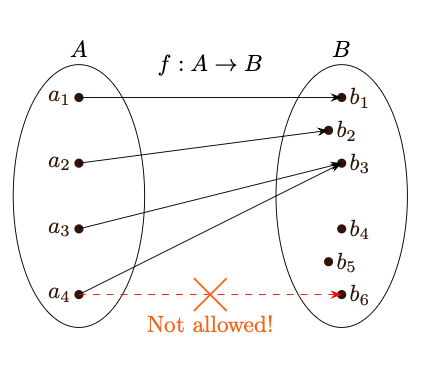
\includegraphics[width=\textwidth/2]{4_func0}
\end{center}


There are also a few common function types that we will define:

\begin{definition}[Injective]
    A function $f: A \rightarrow B$ is injective if $\forall a_1, a_2 \in A$, we have $f(a_1) = f(a_2) \implies a_1 = a_2$.
\end{definition}


\begin{definition}[Surjective]
    A function $f: A \rightarrow B$ is surjective if the whole codomain is covered, meaning that $\forall b \in B, \quad \exists a \in A$ such that $f(a) = b$.
\end{definition}

Sometimes we call surjective functions \emph{onto} functions.

\begin{definition}[Bijective]
    A function is bijective if it is both \emph{injective} and \emph{surjective}.
\end{definition}


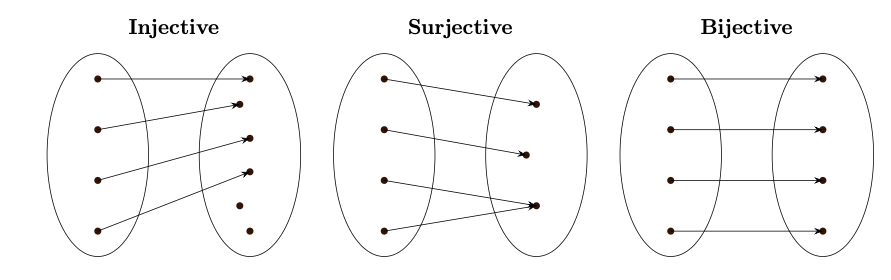
\includegraphics[width=\textwidth]{4_func1}


Only with bijectivity established can we define the inverse of a function.

\begin{definition}[Inverse Function]
    If we take the function $f: A \rightarrow B$, it's domain $A$ and codomain $B$, we can define an inverse function $f^{-1}: B \rightarrow A$ such that $\forall b \in B, \quad f^{-1}(b) = a$ if and only if $f(a) = b$. 
\end{definition}
 
Put plainly, $\forall a \in A, \quad f^{-1}(f(a)) = a$ and $\forall b \in B, \quad f(f^{-1}(b)) = b$.


\subsection{Common Functions and Asymptotic Behavior}

This section will be a brief review of real functions $(f: \mathbb{R} \rightarrow \mathbb{R})$ commonly used in quantum computing. 
\subsubsection*{Power Functions}

Power functions take the form $f(x) = x^p, \quad x \geq 0, p \in \mathbb{R}$. 

The behavior of the function varies significantly with the exponent $p$:

\begin{itemize}
    \item For $p > 0$, $f(x)$ increases as $x$ increases. $f(x)$ exhibits a more rapid growth with a larger $p$.
    
    \item For $p < 0$, $f(x)$ decreases as $x$ increases.
    
    \item When $p = 0$, $f(x) = 1$, regardless of $x$ (excluding $x = 0$), which is a constant function.
    
    \item For $p = 1$, $f(x) = x$, representing a linear relationship.
\end{itemize}

Key properties of power functions include the rules for exponentiation:

\begin{itemize}
    \item Multiplying powers with the same base: $x^a \cdot x^b = x^{a+b}$.
    
    \item Dividing powers with the same base: $x^a / x^b = x^{a-b}$.
\end{itemize}

\subsubsection*{Polynomial Functions}

A polynomial function is a sum of terms $a_i x^i$, where $i$ is a non-negative integer:

\[
f(x) = a_0 + a_1 x + a_2 x^2 + \cdots + a_n x^n.
\]

Its behavior for large $x$ values is predominantly determined by its highest power term, $x^n$, where $n$ is the degree of the polynomial.

An $n$-th degree polynomial has $n$ complex roots (counting multiplicities), and according to Vieta's formulas, the sum of these roots is equal to $-a_{n-1}/a_n$ and their product $(-1)^n a_0/a_n$.

\begin{example}
Consider the polynomial function $f(x) = x^3 - 7x^2 + 14x - 8$. It can be factored as:
\[
f(x) = (x - 1)(x - 2)(x - 4).
\]
\end{example}

The roots of this polynomial are $x = 1, x = 2$, and $x = 4$, which can be found by solving the equations $(x - 1) = 0, (x - 2) = 0$, and $(x - 4) = 0$. According to Vieta's formulas, the sum of the roots is:

\[
1 + 2 + 4 = 7 = -\frac{-7}{1},
\]

and the product is:

\[
1 \cdot 2 \cdot 4 = 8 = (-1)^3 \frac{-8}{1}.
\]

\subsubsection*{Exponential Functions}

Exponential functions are defined as $f(x) = b^x$, where $b$ is a positive constant (called the base) and $b \neq 1$. The variable $x$ is the exponent. The key characteristic is that the variable is in the exponent. Some important notes:

\begin{itemize}
    \item Growth and Decay:
    \begin{itemize}
        \item If $b > 1$, $f(x)$ exhibits exponential growth -- increasing rapidly as $x$ increases. Larger bases lead to faster growth.
        
        \item If $0 < b < 1$, $f(x)$ shows exponential decay -- decreasing towards zero as $x$ increases.
    \end{itemize}
    
    \item Always Positive: Exponential functions are always positive for any real-valued input $x$.
    
    \item Horizontal Asymptote: They approach zero for one direction of $x$ (negative infinity for growth, positive infinity for decay).
    
    \item Base $e$: The natural exponential function with $b = e$ (Euler's number, $\approx 2.718$), i.e, $e^x$, also denoted as $\exp(x)$, has special significance across mathematics.
\end{itemize}

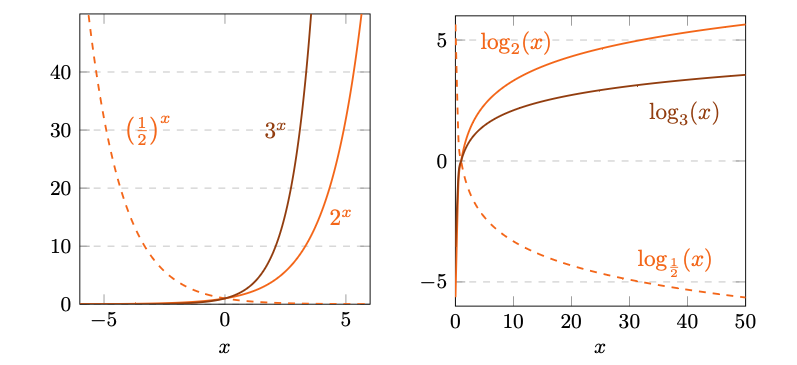
\includegraphics[width=\textwidth]{4_func2}


\subsubsection*{Logarithmic Functions}

Logarithmic functions are the inverses of exponential functions. They are defined as $f(x) = \log_b(x)$, where $b$ is a positive constant $(b \neq 1)$ and $x > 0$. Some key points:

\begin{itemize}
    \item Reversing Exponentiation: If $b^y = x$ then $\log_b(x) = y$.
    
    \item Growth and Behavior
    \begin{itemize}
        \item For $b > 1$, $\log_b(x)$ increases as $x$ increases, but very slowly.
        
        \item For $0 < b < 1$, $\log_b(x)$ decreases as $x$ increases.
    \end{itemize}
    
    \item Vertical Asymptote: Logarithmic functions have a vertical asymptote at $x = 0$.
    
    \item Logarithms of 1 and the Base: $\log_b(1) = 0$ and $\log_b(b) = 1$.
    
    \item The natural logarithm, written as $\ln(x)$ has the base $e$.
\end{itemize}

Key Properties:

\begin{itemize}
    \item The Product Rule: $\log_b(xy) = \log_b(x) + \log_b(y)$
    
    \item Logarithms "Break" Exponents: $\log_b(x^y) = y \cdot \log_b(x)$
    
    \item Changing Bases: $\log_b(x) = \log_a(x) / \log_a(b)$
\end{itemize}

Scaling behavior, especially in the context of data structures and algorithm efficiency, is a significant topic for any computing related fields. It concerns itself with witht he evolution of function curves as the response becomes significantly large. We use the \emph{Big O notation} to describe the behavior of a function $f(x), \quad x \rightarrow \infty$. We say that $f(x)$ is $O(g(x))$ meaning that there is some positive constant $c$ such that the upper bound for complexity growth does not increase faster than $c \cdot g(x)$ for a sufficiently large $x$. 

\begin{example}
    For example, consider $$f(x) = 6x^3 + 2x + 1,$$ we say that $f(x)$ is $O(x^3)$ as $x \rightarrow \infty$, as $X^3$ is the dominant term.  
\end{example}


Most of the common limiting functions are illustrated in the following figure: 

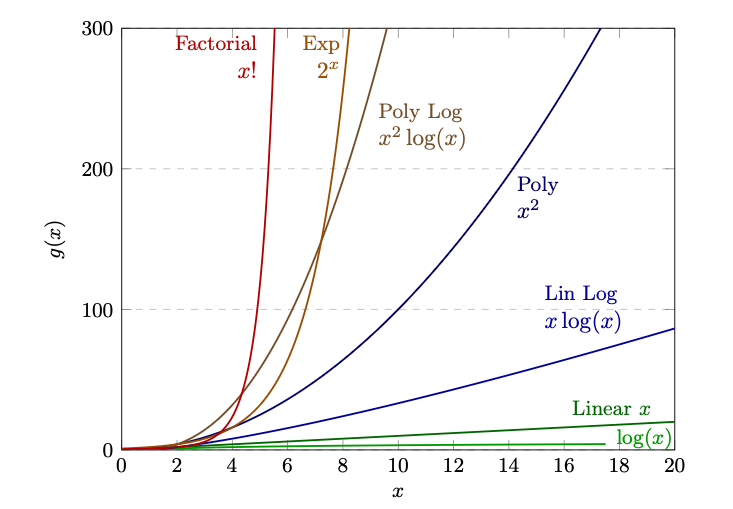
\includegraphics[width=\textwidth]{4_func3}

\begin{enumerate}
    \item Log-log: $g(x) = \log \log(x)$
    \begin{itemize}
        \item Exhibits extremely slow growth. Algorithms within this complexity class increase their running time at a negligible rate with input size escalation.
        
        \item Applications include specialized computational geometry problems.
    \end{itemize}
    
    \item Log: $g(x) = \log(x)$
    \begin{itemize}
        \item Denotes high efficiency. The execution time grows much slower than the input size.
        
        \item Examples include binary search in sorted arrays and operations on certain balanced tree data structures.
    \end{itemize}
    
    \item Sublinear: $g(x) = x^p, 0 < p < 1$
    \begin{itemize}
        \item Exhibits growth slower than linear but faster than logarithmic.
        
        \item Common examples include the Grover's search algorithm in quantum computing, which has a complexity of approximately $O(\sqrt{x})$, and some algorithms that utilize probabilistic methods to achieve faster-than-linear performance on average.
    \end{itemize}
    
    \item Linear: $g(x) = x$
    \begin{itemize}
        \item Indicates direct proportionality. Doubling the input size doubles the running time.
        
        \item Common examples are searching in unsorted lists and identifying max/min elements in a list.
    \end{itemize}
    
    \item Polynomial: $g(x) = x^p, p > 1$
    \begin{itemize}
        \item The growth rate is influenced by the exponent $p$. Higher values lead to rapid increases in running time with input size.
        
        \item Examples: Bubble sort and insertion sort (quadratic complexity), matrix multiplication algorithms (cubic complexity or better).
    \end{itemize}
    
    \item Poly-log: $g(x) = x^p \log(x), p \geq 1$
    \begin{itemize}
        \item Less efficient than the corresponding poly (or linear for $p = 1$) but still considered scalable.
        
        \item Fast Fourier Transform (FFT) algorithms are a prime example of algorithms with linear-log complexity. Some fast sorting algorithms also approach this performance.
    \end{itemize}
    
    \item Exponential: $g(x) = b^x, b > 1$
    \begin{itemize}
        \item Characterized by rapid growth. Algorithms in this class quickly become impractical for moderate input sizes.
        
        \item Examples: Brute-force approaches to the Traveling Salesman Problem. Currently known classical algorithms for integer factorization.
    \end{itemize}
    
    \item Factorial: $g(x) = x!$
    \begin{itemize}
        \item Exhibits extremely rapid growth, surpassing even exponential functions in rate. Practical for only very small input sizes.
        
        \item Example: Generating all permutations of a set.
    \end{itemize}
    
    \item Hyper-exponential: $g(x) = x^x, g(x) = b^{a^x}, g(x) = b^{x!}$, and $g(x) = b^{x^x}$, etc., where $a, b > 1$
    \begin{itemize}
        \item Exhibits growth that is even more rapid than factorial functions.
        
        \item Example: Modeling scenarios with extremely high growth rates, beyond combinatorial complexity.
    \end{itemize}
\end{enumerate}

\break


\section{Vectors and Vector Spaces}

Vectors and the study of vector spaces are fundamental to the study of quantum computing, where they provide the mathmatical framework for representing and manipulating quantum states, commonly used to describe superpositions, entanglement, and other phenomena integral to quantum computing. This section serves as a systematic introduction to the realm of such concepets to lay the foundation for lies ahead. 

\subsection{Real Vectors and Complex Vectors}

A vector is an ordered sequence of numbers. For now, we will focus on vectors with numeric elements. 

\begin{definition}[Ordered $n$-Tuple]
    An ordered sequence of $n$ numbers $(v_1, v_2, \ldots, v_n)$ is called an ordered $n$-tuple. 
\end{definition}

\begin{definition}[Euclidean Space]
    The set comprising all $n$-tuples is called $n$-space or Euclidean space, and denoted as $\mathbb{R}^n$ space. The complex Euclidean space is denoted by $\mathbb{C}^n$ and comprises of all complex $n$-tuples. 
\end{definition}

Now in the context of quantum computing, $n$ is typically finite as we are usually considering finite quantum systems. A real vector is in $\mathbb{R}^n$, while a complex vector is in $\mathbb{C}^n$. Much like $\{\mathbf{0}\}$, we will begin with the defiition of the zero vector.

\begin{definition}[Zero Vector]
    The zero vector, in either $\mathbb{R}^n$ or $\mathbb{C}^n$, denoted by $\{\mathbf{0}\}$, is defined as the vector where all components are zero. $$\{\mathbf{0}\} = (0, 0, \ldots, 0)$$
\end{definition}

While it is difficult to visually represent vectors in higher dimensions, vectors in $\mathbb{R}^2$ and $\mathbb{R}^3$ are easier to represent. Generally, vectors both posess magnitude and direction, conviniently representing force, velocity, and heat flow. They carry weight and direction. 

In linear algebra, vectors with identical length and direction are considered equivalent, unlike vector fields which also consider position, which means that we generally don't draw a distinction between \emph{collinearity} and \emph{parallelism}.

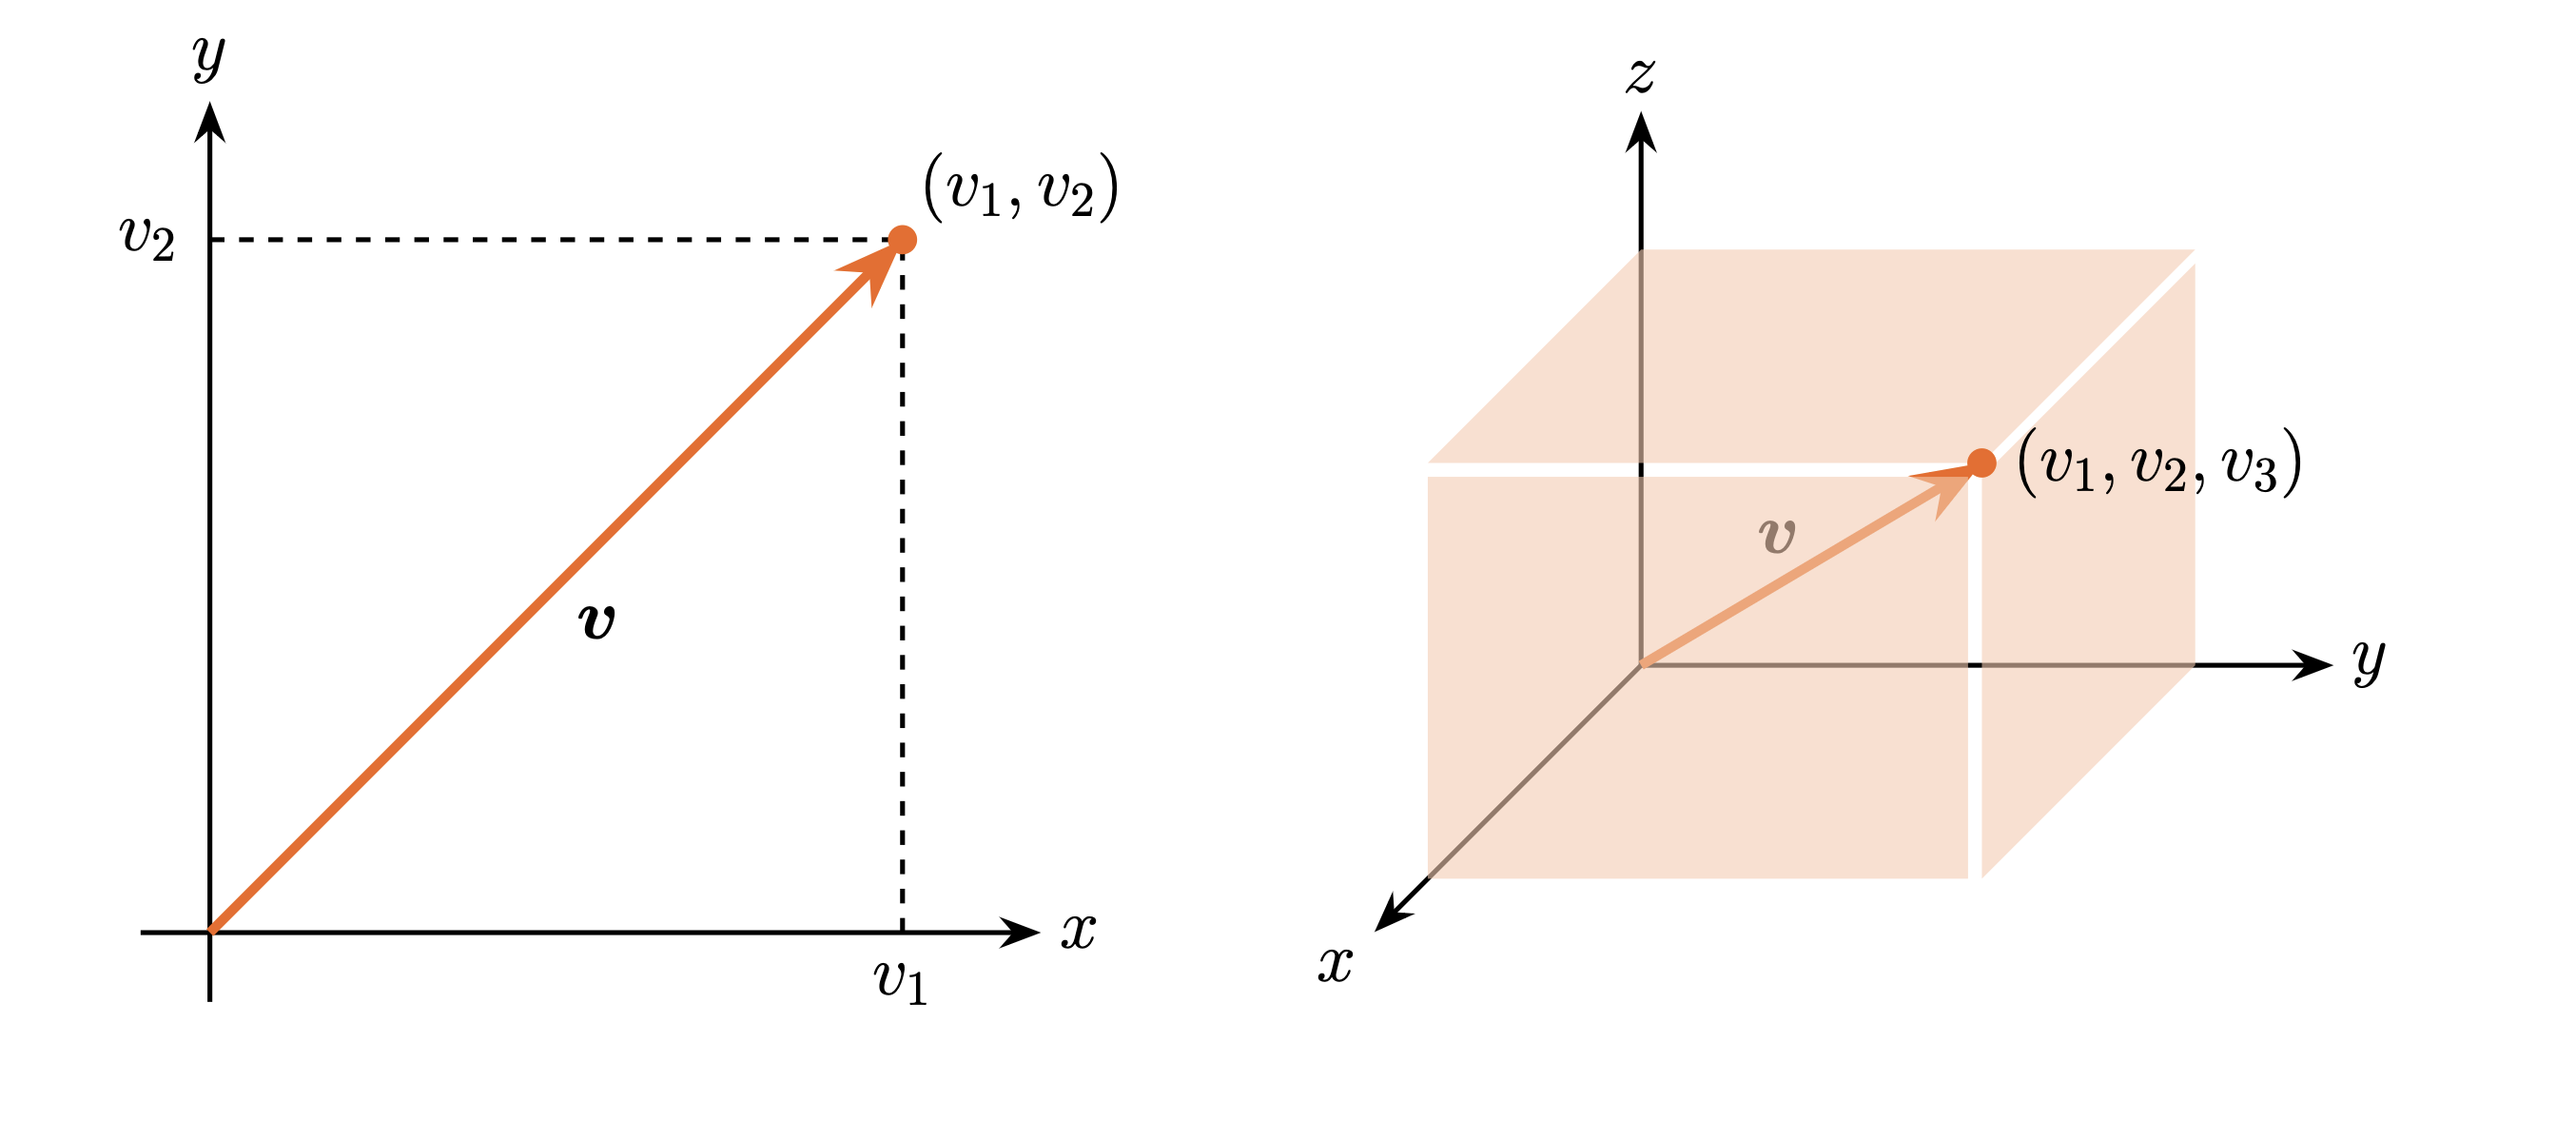
\includegraphics[width=\textwidth]{5_vec0}

While seemingly simple, the intuition from representing vectors in $\mathbb{R}^2$ or $\mathbb{R}^3$ extends to $\mathbb{R}^n, \quad n > 3$ and even $\mathbb{C}^n$, for which geometric applications become exceedingly difficult or near impossible. 



\subsection{Basic Vector Algebra}

A few basic operations on vectors are defined in this subsection in order to establish the foundation of vector manipulation.

\begin{definition}[Vector Equality]
    Given two vectors $\mathbf{u}$ and $\mathbf{v}$ in $\Rn$ or $\Cn$, the two vectors are equal if and only if they are equal element wise. This is also denoted as $\mathbf{u} = \mathbf{v}$.
\end{definition}

For each complex vector, there exists a unique complex conjugate that is defined as follows:

\begin{definition}[Complex Vector Conjugate]
    The complex conjugate of a complex vector $\mathbf{v} = (v_1, v_2, \ldots, v_n)$ is denoted as $\mathbf{v}^*$ and is given by: 
    $$\mathbf{v}^* = (\conj{v_1}, \conj{v_2}, \ldots, \conj{v_n})$$
    Where each element is taken to its complex conjugate.
\end{definition}

Some other common operations also exist for vectors.

\begin{definition}[Vector Sum]
    The sum of two vectors $\mathbf{u}$ and $\mathbf{v}$ in $\Rn$ or $\Cn$ is given by element-wise addition:
    $$\mathbf{u} + \mathbf{v} = (u_1 + v_1, u_2 + v_2, \ldots, u_n + v_n)$$
\end{definition}

While not immediately obvious why this requires a proof, we have 

\begin{theorem}
    Vector addition satisfies the commutative, associative, and identity properties. Mathmatically,
    $$\mathbf{u} + \mathbf{v} = \mathbf{v} + \mathbf{u}$$
    $$\mathbf{u} + (\mathbf{v} + \mathbf{w}) = (\mathbf{u} + \mathbf{v}) + \mathbf{w}$$
    $$\mathbf{v} + \mathbf{0} = \mathbf{v}$$
\end{theorem}


\begin{definition}[Vector Negation]
    The negation of a vector $\mathbf{u}$ in $\Rn$ or $\Cn$ is defined as the element wise negation of $\mathbf{u}$, denoted as $-\mathbf{u}$ and defined as:
    $$-\mathbf{u} = (-v_1, -v_2, \ldots, -v_n)$$
\end{definition}

Which allows us to define vector subtraction. 

\begin{definition}[Vector Subtraction]
    Vector subtraction is defined as adding the negated version of the second vector, also defined as $$\mathbf{u} - \mathbf{v} = \mathbf{u}+ (-\mathbf{v})$$
\end{definition}

Scalar multiplication is also very intuitive, defined as

\begin{definition}
    Given $\mathbf{v}$ in $\Rn$ or $\Cn$ and a scalar $k$, the scalar product is denoted by $k\mathbf{u}$, is defined as:
    $$k\mathbf{v} = (k v_1, k v_2, \ldots, k v_n)$$
\end{definition}

Note that the scalar in this case will usually be from the space in which the vector $\mathbf{v}$ resides. When we combine what we just defined, we have the linear combination. 

\begin{definition}[Linear Combination]
    Consider a vector $\mathbf{w}$ and a set of $r$ vectors $\{\mathbf{v_1}, \mathbf{v_2},$ $ \ldots, \mathbf{v_r}\}$ in $\Rn$ or $\Cn$, we say that $\mathbf{w}$ is a linear combination of $\{\mathbf{v_1}, \mathbf{v_2}, \ldots, \mathbf{v_r}\}$ if $\mathbf{w}$ can be expressed as:
    $$\mathbf{w} = k_1 \mathbf{v_1} + k_2 \mathbf{v_2} + \ldots + k_r \mathbf{v_r} = \sum_{i = 1}^{r} k_i \mathbf{v_i}$$ 
    where each $k_i$ is a scalar, referred to as the \textbf{coefficients} of the linear combination.
\end{definition}

\subsection{Vector Spaces, Subspaces, and Span}

\subsection{Linear Independence, Basis, and Dimension}


















\end{document}